\section{Mesh / xy}
\clearpage\subsection*{M=2: every cache allowance}
\begin{center}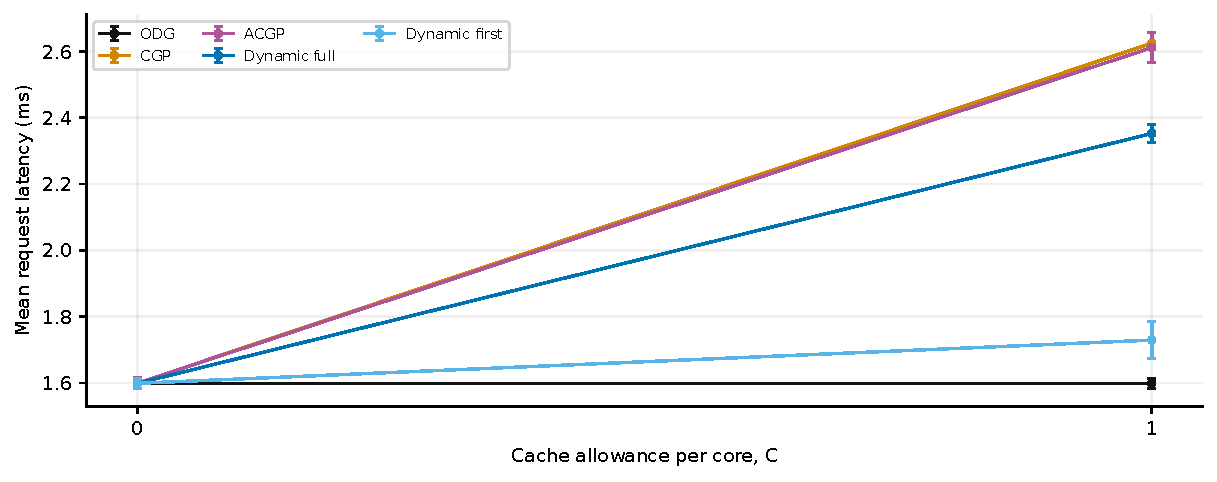
\includegraphics[width=.94\linewidth,height=.31\textheight,keepaspectratio]{figures/allocation/mesh_xy_m2.pdf}\captionof{figure}{All legal C values; ODG's C=0 result is repeated as a horizontal reference, not rerun at C>0.}\end{center}
\begin{center}{\scriptsize\setlength{\tabcolsep}{3pt}
\begin{tabular}{lrrrrr}
\toprule
C & ODG & CGP & ACGP & Dynamic full & Dynamic first \\
\midrule
0 & $1.599\pm0.016$ & $1.598\pm0.016$ & $1.598\pm0.016$ & $1.599\pm0.016$ & $1.599\pm0.016$ \\
1 & $1.599\pm0.016$ & $2.625\pm0.000$ & $2.612\pm0.046$ & $2.353\pm0.026$ & $1.729\pm0.055$ \\
\bottomrule\end{tabular}}
\captionof{table}{Mean hop latency (ms), mean $\pm$ SD. The linked CSV includes every recorded metric for every allocation.}
{\footnotesize\href{https://github.com/sanjeevkrishnaa/Compiler-Driven-ACE/blob/codex/ace-scheduler-correctness/docs/latex/qft96_final/data/allocation_mesh_xy_m2.csv}{Exact CSV values and sample counts}}
\end{center}
\clearpage\subsection*{M=3: every cache allowance}
\begin{center}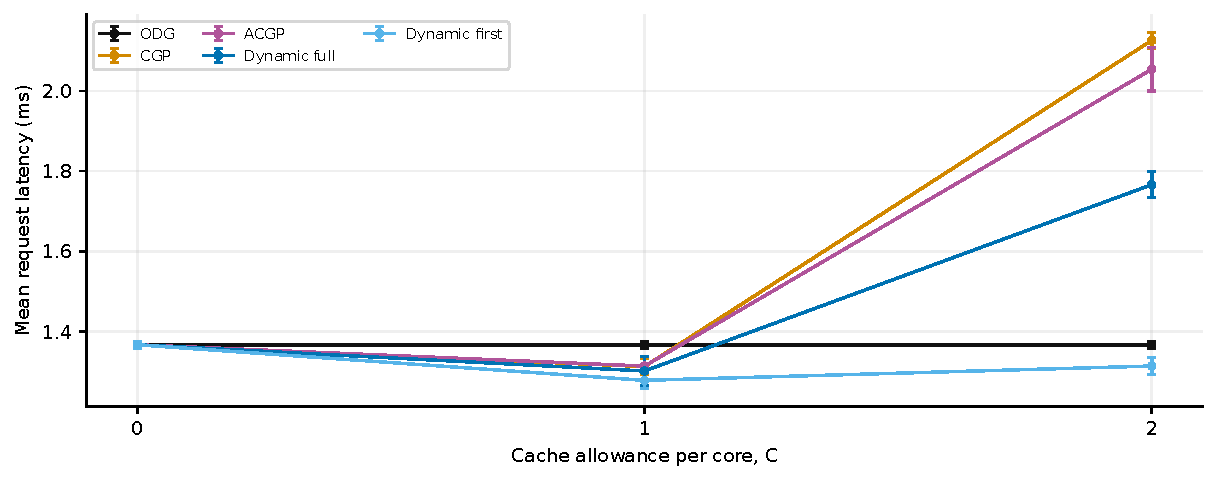
\includegraphics[width=.94\linewidth,height=.31\textheight,keepaspectratio]{figures/allocation/mesh_xy_m3.pdf}\captionof{figure}{All legal C values; ODG's C=0 result is repeated as a horizontal reference, not rerun at C>0.}\end{center}
\begin{center}{\scriptsize\setlength{\tabcolsep}{3pt}
\begin{tabular}{lrrrrr}
\toprule
C & ODG & CGP & ACGP & Dynamic full & Dynamic first \\
\midrule
0 & $1.367\pm0.008$ & $1.367\pm0.007$ & $1.367\pm0.007$ & $1.367\pm0.008$ & $1.367\pm0.008$ \\
1 & $1.367\pm0.008$ & $1.312\pm0.020$ & $1.314\pm0.000$ & $1.301\pm0.035$ & $1.278\pm0.021$ \\
2 & $1.367\pm0.008$ & $2.126\pm0.020$ & $2.054\pm0.054$ & $1.766\pm0.032$ & $1.314\pm0.022$ \\
\bottomrule\end{tabular}}
\captionof{table}{Mean hop latency (ms), mean $\pm$ SD. The linked CSV includes every recorded metric for every allocation.}
{\footnotesize\href{https://github.com/sanjeevkrishnaa/Compiler-Driven-ACE/blob/codex/ace-scheduler-correctness/docs/latex/qft96_final/data/allocation_mesh_xy_m3.csv}{Exact CSV values and sample counts}}
\end{center}
\clearpage\subsection*{M=4: every cache allowance}
\begin{center}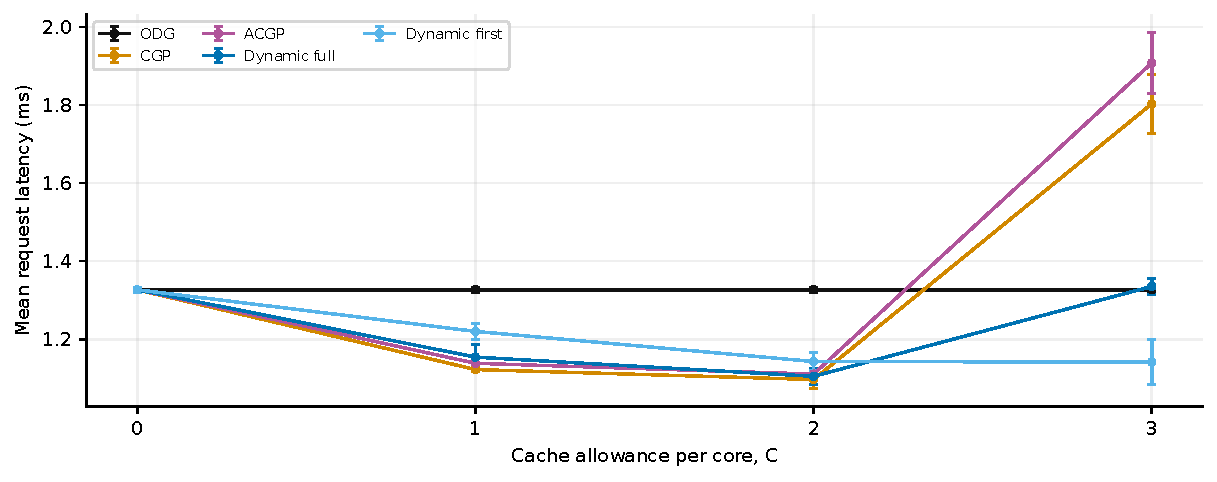
\includegraphics[width=.94\linewidth,height=.31\textheight,keepaspectratio]{figures/allocation/mesh_xy_m4.pdf}\captionof{figure}{All legal C values; ODG's C=0 result is repeated as a horizontal reference, not rerun at C>0.}\end{center}
\begin{center}{\scriptsize\setlength{\tabcolsep}{3pt}
\begin{tabular}{lrrrrr}
\toprule
C & ODG & CGP & ACGP & Dynamic full & Dynamic first \\
\midrule
0 & $1.327\pm0.006$ & $1.327\pm0.006$ & $1.327\pm0.006$ & $1.327\pm0.006$ & $1.327\pm0.006$ \\
1 & $1.327\pm0.006$ & $1.122\pm0.004$ & $1.138\pm0.002$ & $1.154\pm0.032$ & $1.220\pm0.021$ \\
2 & $1.327\pm0.006$ & $1.097\pm0.024$ & $1.110\pm0.007$ & $1.105\pm0.021$ & $1.143\pm0.022$ \\
3 & $1.327\pm0.006$ & $1.803\pm0.075$ & $1.908\pm0.079$ & $1.335\pm0.020$ & $1.141\pm0.058$ \\
\bottomrule\end{tabular}}
\captionof{table}{Mean hop latency (ms), mean $\pm$ SD. The linked CSV includes every recorded metric for every allocation.}
{\footnotesize\href{https://github.com/sanjeevkrishnaa/Compiler-Driven-ACE/blob/codex/ace-scheduler-correctness/docs/latex/qft96_final/data/allocation_mesh_xy_m4.csv}{Exact CSV values and sample counts}}
\end{center}
\clearpage\subsection*{M=6: every cache allowance}
\begin{center}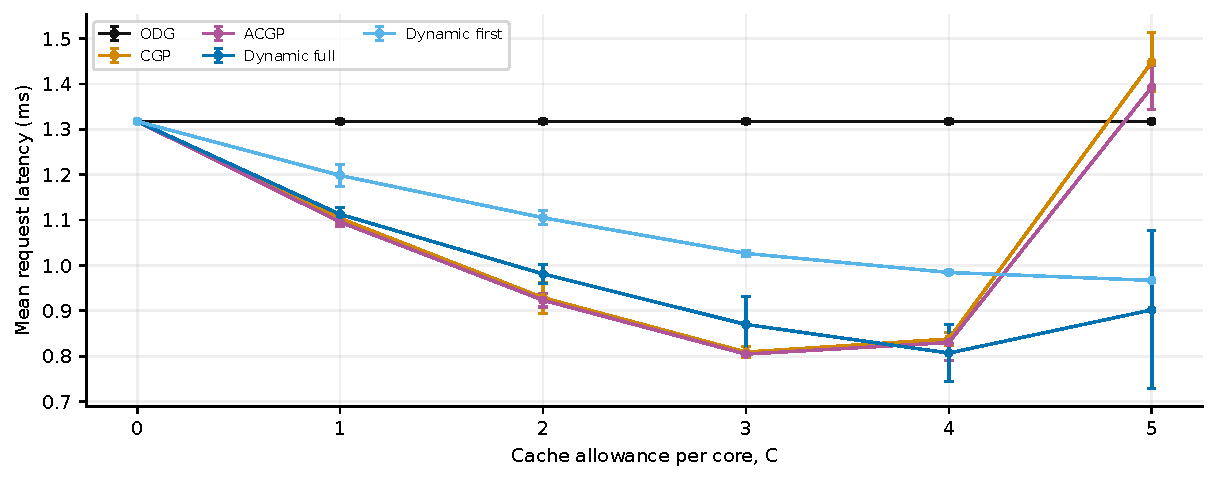
\includegraphics[width=.94\linewidth,height=.31\textheight,keepaspectratio]{figures/allocation/mesh_xy_m6.pdf}\captionof{figure}{All legal C values; ODG's C=0 result is repeated as a horizontal reference, not rerun at C>0.}\end{center}
\begin{center}{\scriptsize\setlength{\tabcolsep}{3pt}
\begin{tabular}{lrrrrr}
\toprule
C & ODG & CGP & ACGP & Dynamic full & Dynamic first \\
\midrule
0 & $1.317\pm0.004$ & $1.318\pm0.004$ & $1.318\pm0.004$ & $1.317\pm0.004$ & $1.317\pm0.004$ \\
1 & $1.317\pm0.004$ & $1.104\pm0.011$ & $1.096\pm0.009$ & $1.113\pm0.016$ & $1.198\pm0.025$ \\
2 & $1.317\pm0.004$ & $0.9290\pm0.0345$ & $0.9234\pm0.0151$ & $0.9813\pm0.0201$ & $1.105\pm0.015$ \\
3 & $1.317\pm0.004$ & $0.8091\pm0.0118$ & $0.8045\pm0.0028$ & $0.8700\pm0.0613$ & $1.026\pm0.006$ \\
4 & $1.317\pm0.004$ & $0.8379\pm0.0139$ & $0.8301\pm0.0394$ & $0.8070\pm0.0620$ & $0.9846\pm0.0032$ \\
5 & $1.317\pm0.004$ & $1.448\pm0.066$ & $1.393\pm0.049$ & $0.9021\pm0.1738$ & $0.9670\pm0.0025$ \\
\bottomrule\end{tabular}}
\captionof{table}{Mean hop latency (ms), mean $\pm$ SD. The linked CSV includes every recorded metric for every allocation.}
{\footnotesize\href{https://github.com/sanjeevkrishnaa/Compiler-Driven-ACE/blob/codex/ace-scheduler-correctness/docs/latex/qft96_final/data/allocation_mesh_xy_m6.csv}{Exact CSV values and sample counts}}
\end{center}
\clearpage\subsection*{M=8: every cache allowance}
\begin{center}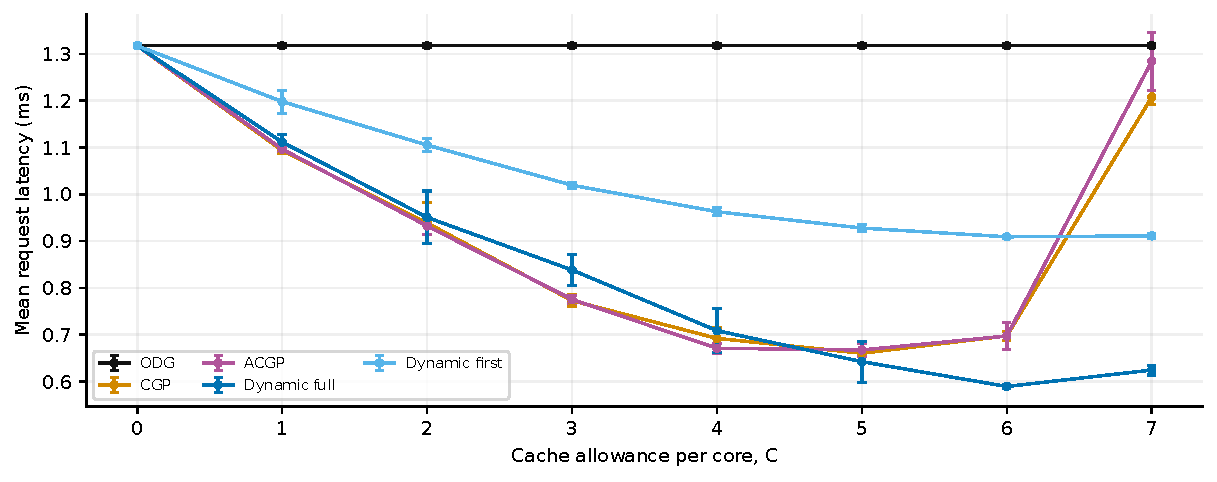
\includegraphics[width=.94\linewidth,height=.31\textheight,keepaspectratio]{figures/allocation/mesh_xy_m8.pdf}\captionof{figure}{All legal C values; ODG's C=0 result is repeated as a horizontal reference, not rerun at C>0.}\end{center}
\begin{center}{\scriptsize\setlength{\tabcolsep}{3pt}
\begin{tabular}{lrrrrr}
\toprule
C & ODG & CGP & ACGP & Dynamic full & Dynamic first \\
\midrule
0 & $1.317\pm0.004$ & $1.318\pm0.004$ & $1.318\pm0.004$ & $1.317\pm0.004$ & $1.317\pm0.004$ \\
1 & $1.317\pm0.004$ & $1.094\pm0.007$ & $1.097\pm0.005$ & $1.112\pm0.017$ & $1.198\pm0.025$ \\
2 & $1.317\pm0.004$ & $0.9386\pm0.0438$ & $0.9324\pm0.0183$ & $0.9507\pm0.0564$ & $1.105\pm0.013$ \\
3 & $1.317\pm0.004$ & $0.7729\pm0.0124$ & $0.7754\pm0.0091$ & $0.8382\pm0.0332$ & $1.019\pm0.006$ \\
4 & $1.317\pm0.004$ & $0.6921\pm0.0226$ & $0.6710\pm0.0108$ & $0.7086\pm0.0472$ & $0.9628\pm0.0086$ \\
5 & $1.317\pm0.004$ & $0.6604\pm0.0015$ & $0.6674\pm0.0142$ & $0.6423\pm0.0441$ & $0.9278\pm0.0076$ \\
6 & $1.317\pm0.004$ & $0.6975\pm0.0095$ & $0.6972\pm0.0297$ & $0.5893\pm0.0049$ & $0.9092\pm0.0032$ \\
7 & $1.317\pm0.004$ & $1.208\pm0.015$ & $1.284\pm0.062$ & $0.6244\pm0.0106$ & $0.9111\pm0.0051$ \\
\bottomrule\end{tabular}}
\captionof{table}{Mean hop latency (ms), mean $\pm$ SD. The linked CSV includes every recorded metric for every allocation.}
{\footnotesize\href{https://github.com/sanjeevkrishnaa/Compiler-Driven-ACE/blob/codex/ace-scheduler-correctness/docs/latex/qft96_final/data/allocation_mesh_xy_m8.csv}{Exact CSV values and sample counts}}
\end{center}
\clearpage\subsection*{M=16: every cache allowance}
\begin{center}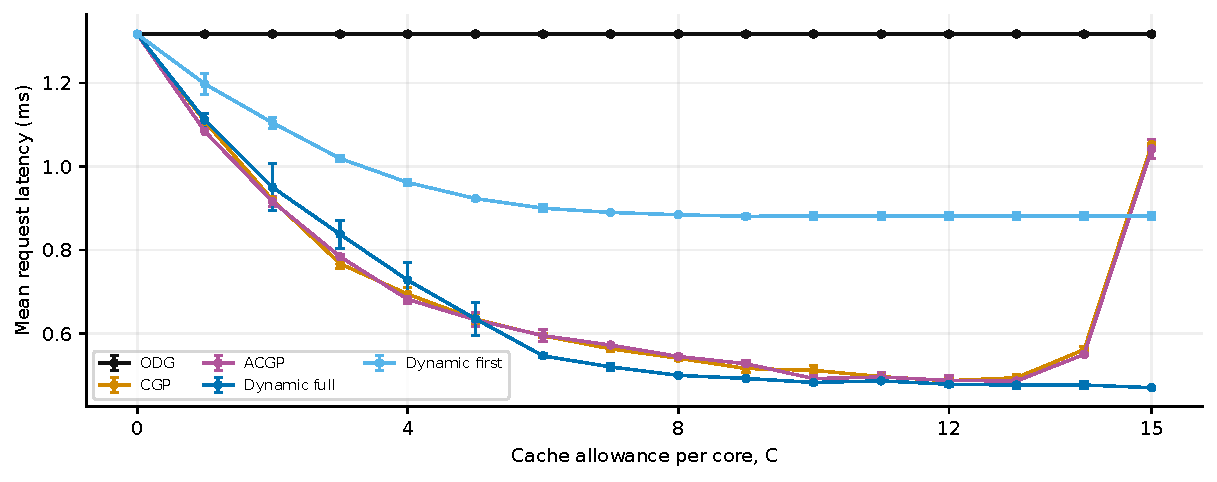
\includegraphics[width=.94\linewidth,height=.31\textheight,keepaspectratio]{figures/allocation/mesh_xy_m16.pdf}\captionof{figure}{All legal C values; ODG's C=0 result is repeated as a horizontal reference, not rerun at C>0.}\end{center}
\begin{center}{\scriptsize\setlength{\tabcolsep}{3pt}
\begin{tabular}{lrrrrr}
\toprule
C & ODG & CGP & ACGP & Dynamic full & Dynamic first \\
\midrule
0 & $1.317\pm0.004$ & $1.318\pm0.004$ & $1.318\pm0.004$ & $1.317\pm0.004$ & $1.317\pm0.004$ \\
1 & $1.317\pm0.004$ & $1.108\pm0.001$ & $1.084\pm0.000$ & $1.112\pm0.017$ & $1.198\pm0.025$ \\
2 & $1.317\pm0.004$ & $0.9202\pm0.0057$ & $0.9164\pm0.0116$ & $0.9507\pm0.0564$ & $1.105\pm0.013$ \\
3 & $1.317\pm0.004$ & $0.7674\pm0.0106$ & $0.7843\pm0.0060$ & $0.8380\pm0.0332$ & $1.019\pm0.006$ \\
4 & $1.317\pm0.004$ & $0.6945\pm0.0149$ & $0.6819\pm0.0096$ & $0.7281\pm0.0428$ & $0.9620\pm0.0082$ \\
5 & $1.317\pm0.004$ & $0.6347\pm0.0129$ & $0.6332\pm0.0168$ & $0.6353\pm0.0391$ & $0.9236\pm0.0035$ \\
6 & $1.317\pm0.004$ & $0.5950\pm0.0053$ & $0.5952\pm0.0136$ & $0.5468\pm0.0045$ & $0.9003\pm0.0077$ \\
7 & $1.317\pm0.004$ & $0.5636\pm0.0074$ & $0.5726\pm0.0003$ & $0.5201\pm0.0086$ & $0.8902\pm0.0020$ \\
8 & $1.317\pm0.004$ & $0.5411\pm0.0049$ & $0.5452\pm0.0043$ & $0.5000\pm0.0037$ & $0.8847\pm0.0017$ \\
9 & $1.317\pm0.004$ & $0.5164\pm0.0089$ & $0.5279\pm0.0082$ & $0.4925\pm0.0005$ & $0.8809\pm0.0041$ \\
10 & $1.317\pm0.004$ & $0.5121\pm0.0109$ & $0.4923\pm0.0073$ & $0.4831\pm0.0054$ & $0.8823\pm0.0078$ \\
11 & $1.317\pm0.004$ & $0.4969\pm0.0074$ & $0.4961\pm0.0115$ & $0.4868\pm0.0017$ & $0.8823\pm0.0078$ \\
12 & $1.317\pm0.004$ & $0.4872\pm0.0051$ & $0.4879\pm0.0123$ & $0.4787\pm0.0053$ & $0.8823\pm0.0078$ \\
13 & $1.317\pm0.004$ & $0.4944\pm0.0073$ & $0.4864\pm0.0013$ & $0.4767\pm0.0072$ & $0.8823\pm0.0078$ \\
14 & $1.317\pm0.004$ & $0.5616\pm0.0067$ & $0.5503\pm0.0027$ & $0.4770\pm0.0090$ & $0.8823\pm0.0078$ \\
15 & $1.317\pm0.004$ & $1.053\pm0.011$ & $1.042\pm0.023$ & $0.4705\pm0.0020$ & $0.8823\pm0.0078$ \\
\bottomrule\end{tabular}}
\captionof{table}{Mean hop latency (ms), mean $\pm$ SD. The linked CSV includes every recorded metric for every allocation.}
{\footnotesize\href{https://github.com/sanjeevkrishnaa/Compiler-Driven-ACE/blob/codex/ace-scheduler-correctness/docs/latex/qft96_final/data/allocation_mesh_xy_m16.csv}{Exact CSV values and sample counts}}
\end{center}
\clearpage\subsection*{M=32: every cache allowance}
\begin{center}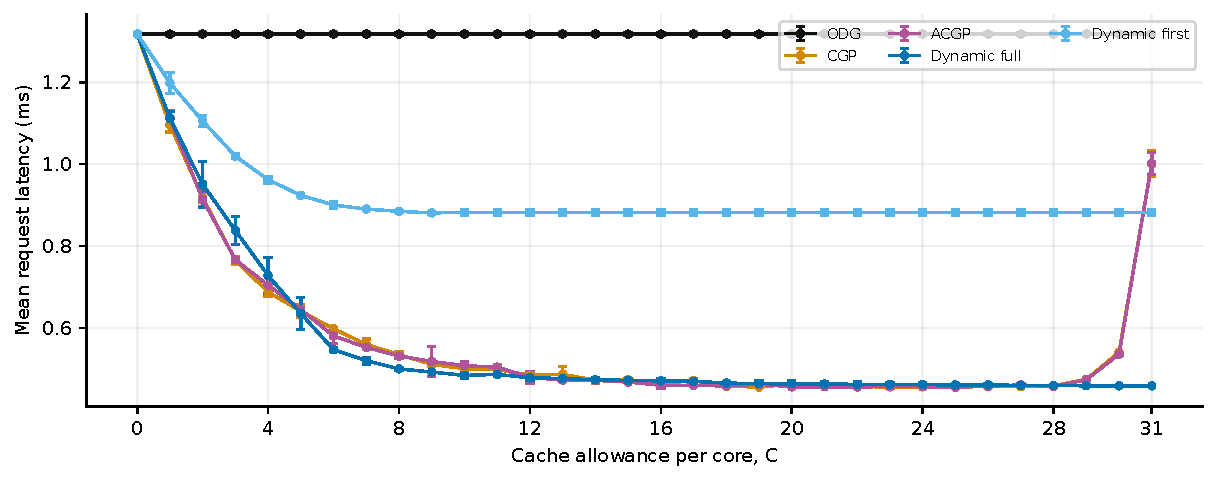
\includegraphics[width=.94\linewidth,height=.31\textheight,keepaspectratio]{figures/allocation/mesh_xy_m32.pdf}\captionof{figure}{All legal C values; ODG's C=0 result is repeated as a horizontal reference, not rerun at C>0.}\end{center}
\begin{center}{\scriptsize\setlength{\tabcolsep}{3pt}
\begin{tabular}{lrrrrr}
\toprule
C & ODG & CGP & ACGP & Dynamic full & Dynamic first \\
\midrule
0 & $1.317\pm0.004$ & $1.318\pm0.004$ & $1.318\pm0.004$ & $1.317\pm0.004$ & $1.317\pm0.004$ \\
1 & $1.317\pm0.004$ & $1.096\pm0.017$ & $1.112\pm0.018$ & $1.112\pm0.017$ & $1.198\pm0.025$ \\
2 & $1.317\pm0.004$ & $0.9183\pm0.0116$ & $0.9139\pm0.0182$ & $0.9507\pm0.0564$ & $1.105\pm0.013$ \\
3 & $1.317\pm0.004$ & $0.7653\pm0.0099$ & $0.7664\pm0.0002$ & $0.8380\pm0.0332$ & $1.019\pm0.006$ \\
4 & $1.317\pm0.004$ & $0.6877\pm0.0116$ & $0.7045\pm0.0063$ & $0.7281\pm0.0428$ & $0.9620\pm0.0082$ \\
5 & $1.317\pm0.004$ & $0.6410\pm0.0163$ & $0.6450\pm0.0057$ & $0.6353\pm0.0391$ & $0.9236\pm0.0035$ \\
6 & $1.317\pm0.004$ & $0.5980\pm0.0017$ & $0.5806\pm0.0195$ & $0.5468\pm0.0045$ & $0.9003\pm0.0077$ \\
7 & $1.317\pm0.004$ & $0.5599\pm0.0131$ & $0.5527\pm0.0028$ & $0.5201\pm0.0086$ & $0.8902\pm0.0020$ \\
8 & $1.317\pm0.004$ & $0.5349\pm0.0084$ & $0.5315\pm0.0060$ & $0.5000\pm0.0037$ & $0.8847\pm0.0017$ \\
9 & $1.317\pm0.004$ & $0.5113\pm0.0059$ & $0.5182\pm0.0373$ & $0.4925\pm0.0005$ & $0.8809\pm0.0041$ \\
10 & $1.317\pm0.004$ & $0.5005\pm0.0064$ & $0.5078\pm0.0101$ & $0.4841\pm0.0069$ & $0.8823\pm0.0078$ \\
11 & $1.317\pm0.004$ & $0.4986\pm0.0110$ & $0.5044\pm0.0005$ & $0.4868\pm0.0017$ & $0.8823\pm0.0078$ \\
12 & $1.317\pm0.004$ & $0.4845\pm0.0088$ & $0.4797\pm0.0142$ & $0.4782\pm0.0059$ & $0.8823\pm0.0078$ \\
13 & $1.317\pm0.004$ & $0.4867\pm0.0183$ & $0.4726\pm0.0001$ & $0.4767\pm0.0072$ & $0.8823\pm0.0078$ \\
14 & $1.317\pm0.004$ & $0.4725\pm0.0072$ & $0.4722\pm0.0039$ & $0.4734\pm0.0051$ & $0.8823\pm0.0078$ \\
15 & $1.317\pm0.004$ & $0.4736\pm0.0019$ & $0.4680\pm0.0003$ & $0.4720\pm0.0043$ & $0.8823\pm0.0078$ \\
16 & $1.317\pm0.004$ & $0.4656\pm0.0072$ & $0.4600\pm0.0084$ & $0.4709\pm0.0053$ & $0.8823\pm0.0078$ \\
17 & $1.317\pm0.004$ & $0.4709\pm0.0052$ & $0.4602\pm0.0018$ & $0.4698\pm0.0051$ & $0.8823\pm0.0078$ \\
18 & $1.317\pm0.004$ & $0.4578\pm0.0020$ & $0.4583\pm0.0019$ & $0.4656\pm0.0048$ & $0.8823\pm0.0078$ \\
19 & $1.317\pm0.004$ & $0.4558\pm0.0001$ & $0.4630\pm0.0010$ & $0.4639\pm0.0073$ & $0.8823\pm0.0078$ \\
20 & $1.317\pm0.004$ & $0.4627\pm0.0028$ & $0.4561\pm0.0003$ & $0.4636\pm0.0076$ & $0.8823\pm0.0078$ \\
21 & $1.317\pm0.004$ & $0.4566\pm0.0030$ & $0.4564\pm0.0016$ & $0.4633\pm0.0071$ & $0.8823\pm0.0078$ \\
22 & $1.317\pm0.004$ & $0.4570\pm0.0026$ & $0.4560\pm0.0001$ & $0.4624\pm0.0058$ & $0.8823\pm0.0078$ \\
23 & $1.317\pm0.004$ & $0.4561\pm0.0001$ & $0.4571\pm0.0037$ & $0.4622\pm0.0056$ & $0.8823\pm0.0078$ \\
24 & $1.317\pm0.004$ & $0.4563\pm0.0008$ & $0.4568\pm0.0009$ & $0.4616\pm0.0047$ & $0.8823\pm0.0078$ \\
25 & $1.317\pm0.004$ & $0.4560\pm0.0020$ & $0.4555\pm0.0021$ & $0.4611\pm0.0041$ & $0.8823\pm0.0078$ \\
26 & $1.317\pm0.004$ & $0.4570\pm0.0021$ & $0.4578\pm0.0016$ & $0.4610\pm0.0038$ & $0.8823\pm0.0078$ \\
27 & $1.317\pm0.004$ & $0.4568\pm0.0004$ & $0.4609\pm0.0044$ & $0.4597\pm0.0021$ & $0.8823\pm0.0078$ \\
28 & $1.317\pm0.004$ & $0.4589\pm0.0001$ & $0.4569\pm0.0012$ & $0.4596\pm0.0019$ & $0.8823\pm0.0078$ \\
29 & $1.317\pm0.004$ & $0.4744\pm0.0008$ & $0.4738\pm0.0007$ & $0.4588\pm0.0007$ & $0.8823\pm0.0078$ \\
30 & $1.317\pm0.004$ & $0.5408\pm0.0002$ & $0.5358\pm0.0031$ & $0.4587\pm0.0006$ & $0.8823\pm0.0078$ \\
31 & $1.317\pm0.004$ & $1.001\pm0.032$ & $1.002\pm0.028$ & $0.4587\pm0.0006$ & $0.8823\pm0.0078$ \\
\bottomrule\end{tabular}}
\captionof{table}{Mean hop latency (ms), mean $\pm$ SD. The linked CSV includes every recorded metric for every allocation.}
{\footnotesize\href{https://github.com/sanjeevkrishnaa/Compiler-Driven-ACE/blob/codex/ace-scheduler-correctness/docs/latex/qft96_final/data/allocation_mesh_xy_m32.csv}{Exact CSV values and sample counts}}
\end{center}
\section{Mesh / yx}
\clearpage\subsection*{M=2: every cache allowance}
\begin{center}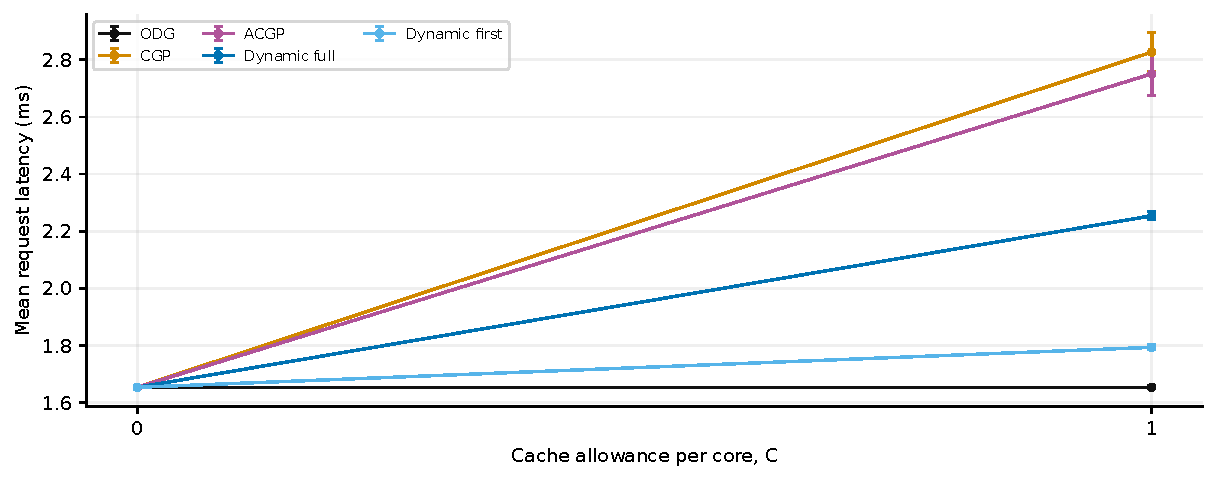
\includegraphics[width=.94\linewidth,height=.31\textheight,keepaspectratio]{figures/allocation/mesh_yx_m2.pdf}\captionof{figure}{All legal C values; ODG's C=0 result is repeated as a horizontal reference, not rerun at C>0.}\end{center}
\begin{center}{\scriptsize\setlength{\tabcolsep}{3pt}
\begin{tabular}{lrrrrr}
\toprule
C & ODG & CGP & ACGP & Dynamic full & Dynamic first \\
\midrule
0 & $1.653\pm0.005$ & $1.653\pm0.005$ & $1.653\pm0.005$ & $1.653\pm0.005$ & $1.653\pm0.005$ \\
1 & $1.653\pm0.005$ & $2.827\pm0.069$ & $2.751\pm0.076$ & $2.254\pm0.014$ & $1.793\pm0.008$ \\
\bottomrule\end{tabular}}
\captionof{table}{Mean hop latency (ms), mean $\pm$ SD. The linked CSV includes every recorded metric for every allocation.}
{\footnotesize\href{https://github.com/sanjeevkrishnaa/Compiler-Driven-ACE/blob/codex/ace-scheduler-correctness/docs/latex/qft96_final/data/allocation_mesh_yx_m2.csv}{Exact CSV values and sample counts}}
\end{center}
\clearpage\subsection*{M=3: every cache allowance}
\begin{center}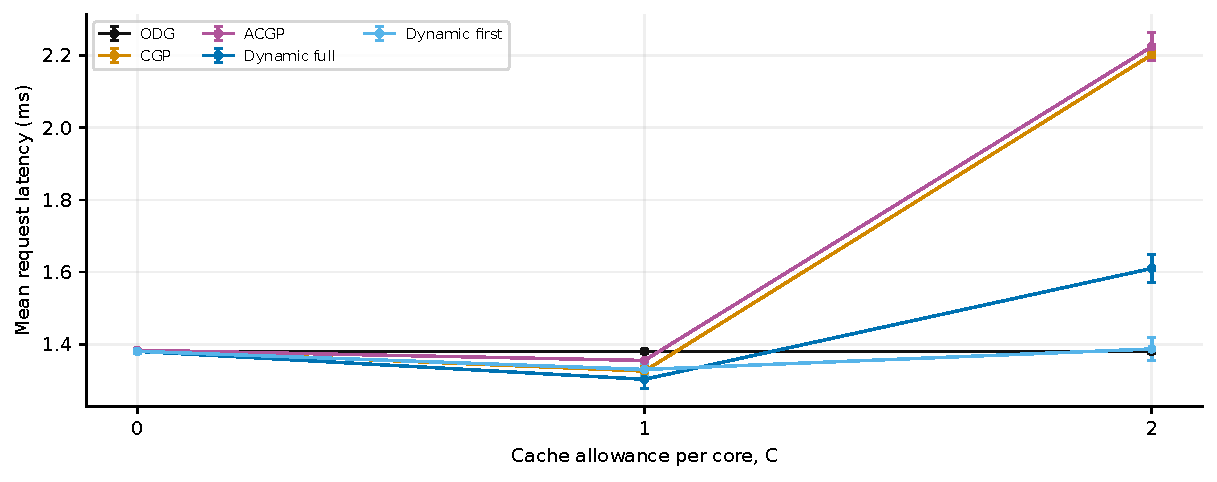
\includegraphics[width=.94\linewidth,height=.31\textheight,keepaspectratio]{figures/allocation/mesh_yx_m3.pdf}\captionof{figure}{All legal C values; ODG's C=0 result is repeated as a horizontal reference, not rerun at C>0.}\end{center}
\begin{center}{\scriptsize\setlength{\tabcolsep}{3pt}
\begin{tabular}{lrrrrr}
\toprule
C & ODG & CGP & ACGP & Dynamic full & Dynamic first \\
\midrule
0 & $1.381\pm0.005$ & $1.384\pm0.001$ & $1.384\pm0.001$ & $1.381\pm0.005$ & $1.381\pm0.005$ \\
1 & $1.381\pm0.005$ & $1.326\pm0.015$ & $1.355\pm0.023$ & $1.303\pm0.026$ & $1.330\pm0.016$ \\
2 & $1.381\pm0.005$ & $2.202\pm0.010$ & $2.224\pm0.040$ & $1.610\pm0.038$ & $1.387\pm0.033$ \\
\bottomrule\end{tabular}}
\captionof{table}{Mean hop latency (ms), mean $\pm$ SD. The linked CSV includes every recorded metric for every allocation.}
{\footnotesize\href{https://github.com/sanjeevkrishnaa/Compiler-Driven-ACE/blob/codex/ace-scheduler-correctness/docs/latex/qft96_final/data/allocation_mesh_yx_m3.csv}{Exact CSV values and sample counts}}
\end{center}
\clearpage\subsection*{M=4: every cache allowance}
\begin{center}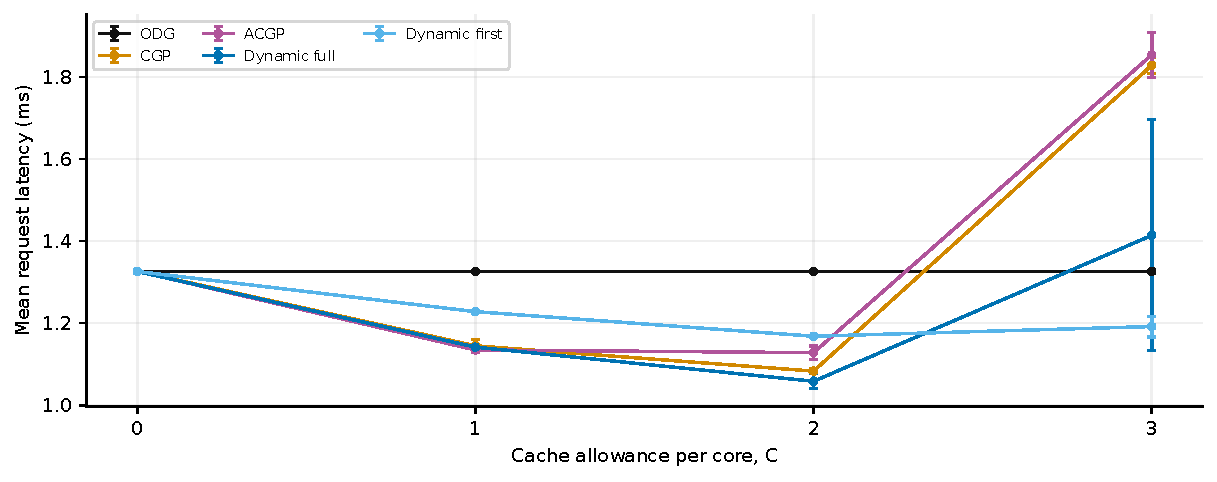
\includegraphics[width=.94\linewidth,height=.31\textheight,keepaspectratio]{figures/allocation/mesh_yx_m4.pdf}\captionof{figure}{All legal C values; ODG's C=0 result is repeated as a horizontal reference, not rerun at C>0.}\end{center}
\begin{center}{\scriptsize\setlength{\tabcolsep}{3pt}
\begin{tabular}{lrrrrr}
\toprule
C & ODG & CGP & ACGP & Dynamic full & Dynamic first \\
\midrule
0 & $1.326\pm0.001$ & $1.327\pm0.002$ & $1.327\pm0.002$ & $1.326\pm0.001$ & $1.326\pm0.001$ \\
1 & $1.326\pm0.001$ & $1.145\pm0.015$ & $1.135\pm0.006$ & $1.142\pm0.001$ & $1.228\pm0.002$ \\
2 & $1.326\pm0.001$ & $1.083\pm0.006$ & $1.128\pm0.016$ & $1.058\pm0.018$ & $1.168\pm0.000$ \\
3 & $1.326\pm0.001$ & $1.828\pm0.019$ & $1.854\pm0.055$ & $1.414\pm0.282$ & $1.192\pm0.025$ \\
\bottomrule\end{tabular}}
\captionof{table}{Mean hop latency (ms), mean $\pm$ SD. The linked CSV includes every recorded metric for every allocation.}
{\footnotesize\href{https://github.com/sanjeevkrishnaa/Compiler-Driven-ACE/blob/codex/ace-scheduler-correctness/docs/latex/qft96_final/data/allocation_mesh_yx_m4.csv}{Exact CSV values and sample counts}}
\end{center}
\clearpage\subsection*{M=6: every cache allowance}
\begin{center}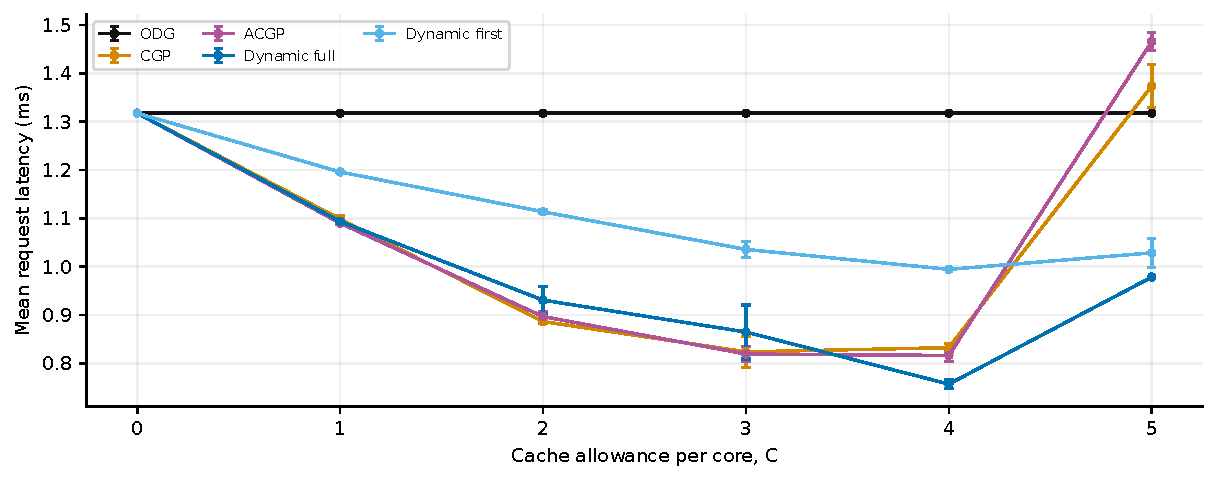
\includegraphics[width=.94\linewidth,height=.31\textheight,keepaspectratio]{figures/allocation/mesh_yx_m6.pdf}\captionof{figure}{All legal C values; ODG's C=0 result is repeated as a horizontal reference, not rerun at C>0.}\end{center}
\begin{center}{\scriptsize\setlength{\tabcolsep}{3pt}
\begin{tabular}{lrrrrr}
\toprule
C & ODG & CGP & ACGP & Dynamic full & Dynamic first \\
\midrule
0 & $1.318\pm0.000$ & $1.318\pm0.000$ & $1.318\pm0.000$ & $1.318\pm0.000$ & $1.318\pm0.000$ \\
1 & $1.318\pm0.000$ & $1.099\pm0.008$ & $1.090\pm0.003$ & $1.094\pm0.002$ & $1.196\pm0.001$ \\
2 & $1.318\pm0.000$ & $0.8866\pm0.0043$ & $0.8968\pm0.0113$ & $0.9308\pm0.0282$ & $1.114\pm0.004$ \\
3 & $1.318\pm0.000$ & $0.8238\pm0.0322$ & $0.8193\pm0.0149$ & $0.8648\pm0.0558$ & $1.036\pm0.017$ \\
4 & $1.318\pm0.000$ & $0.8325\pm0.0092$ & $0.8164\pm0.0127$ & $0.7570\pm0.0096$ & $0.9944\pm0.0010$ \\
5 & $1.318\pm0.000$ & $1.374\pm0.044$ & $1.466\pm0.019$ & $0.9785\pm0.0017$ & $1.029\pm0.030$ \\
\bottomrule\end{tabular}}
\captionof{table}{Mean hop latency (ms), mean $\pm$ SD. The linked CSV includes every recorded metric for every allocation.}
{\footnotesize\href{https://github.com/sanjeevkrishnaa/Compiler-Driven-ACE/blob/codex/ace-scheduler-correctness/docs/latex/qft96_final/data/allocation_mesh_yx_m6.csv}{Exact CSV values and sample counts}}
\end{center}
\clearpage\subsection*{M=8: every cache allowance}
\begin{center}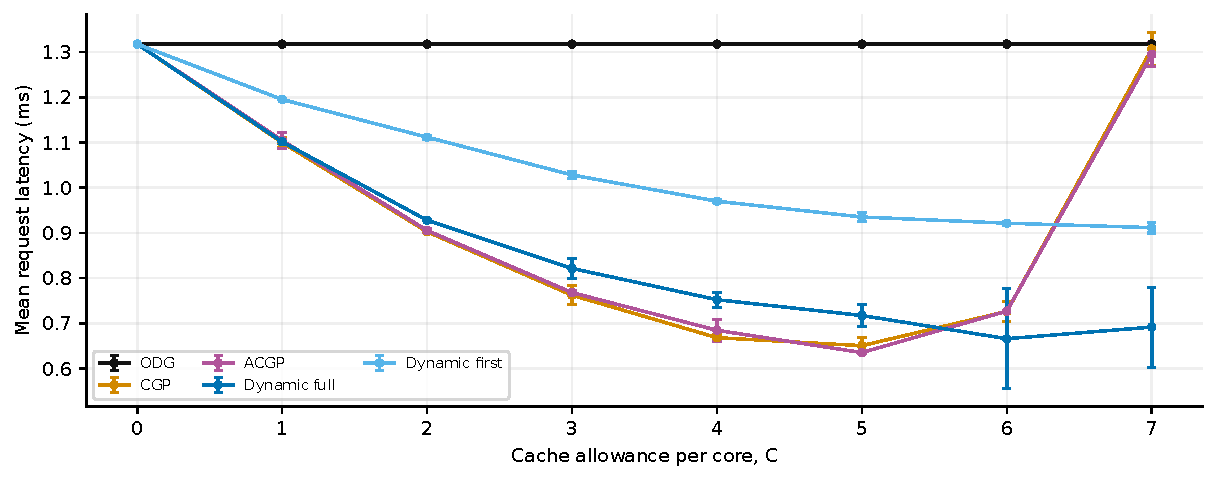
\includegraphics[width=.94\linewidth,height=.31\textheight,keepaspectratio]{figures/allocation/mesh_yx_m8.pdf}\captionof{figure}{All legal C values; ODG's C=0 result is repeated as a horizontal reference, not rerun at C>0.}\end{center}
\begin{center}{\scriptsize\setlength{\tabcolsep}{3pt}
\begin{tabular}{lrrrrr}
\toprule
C & ODG & CGP & ACGP & Dynamic full & Dynamic first \\
\midrule
0 & $1.318\pm0.000$ & $1.318\pm0.000$ & $1.318\pm0.000$ & $1.318\pm0.000$ & $1.318\pm0.000$ \\
1 & $1.318\pm0.000$ & $1.100\pm0.011$ & $1.104\pm0.018$ & $1.101\pm0.004$ & $1.195\pm0.000$ \\
2 & $1.318\pm0.000$ & $0.9026\pm0.0018$ & $0.9053\pm0.0040$ & $0.9279\pm0.0012$ & $1.112\pm0.004$ \\
3 & $1.318\pm0.000$ & $0.7621\pm0.0213$ & $0.7679\pm0.0038$ & $0.8214\pm0.0217$ & $1.028\pm0.007$ \\
4 & $1.318\pm0.000$ & $0.6682\pm0.0062$ & $0.6844\pm0.0245$ & $0.7522\pm0.0169$ & $0.9700\pm0.0034$ \\
5 & $1.318\pm0.000$ & $0.6505\pm0.0181$ & $0.6352\pm0.0025$ & $0.7172\pm0.0236$ & $0.9351\pm0.0103$ \\
6 & $1.318\pm0.000$ & $0.7263\pm0.0216$ & $0.7268\pm0.0009$ & $0.6659\pm0.1106$ & $0.9214\pm0.0042$ \\
7 & $1.318\pm0.000$ & $1.307\pm0.037$ & $1.295\pm0.026$ & $0.6916\pm0.0885$ & $0.9115\pm0.0118$ \\
\bottomrule\end{tabular}}
\captionof{table}{Mean hop latency (ms), mean $\pm$ SD. The linked CSV includes every recorded metric for every allocation.}
{\footnotesize\href{https://github.com/sanjeevkrishnaa/Compiler-Driven-ACE/blob/codex/ace-scheduler-correctness/docs/latex/qft96_final/data/allocation_mesh_yx_m8.csv}{Exact CSV values and sample counts}}
\end{center}
\clearpage\subsection*{M=16: every cache allowance}
\begin{center}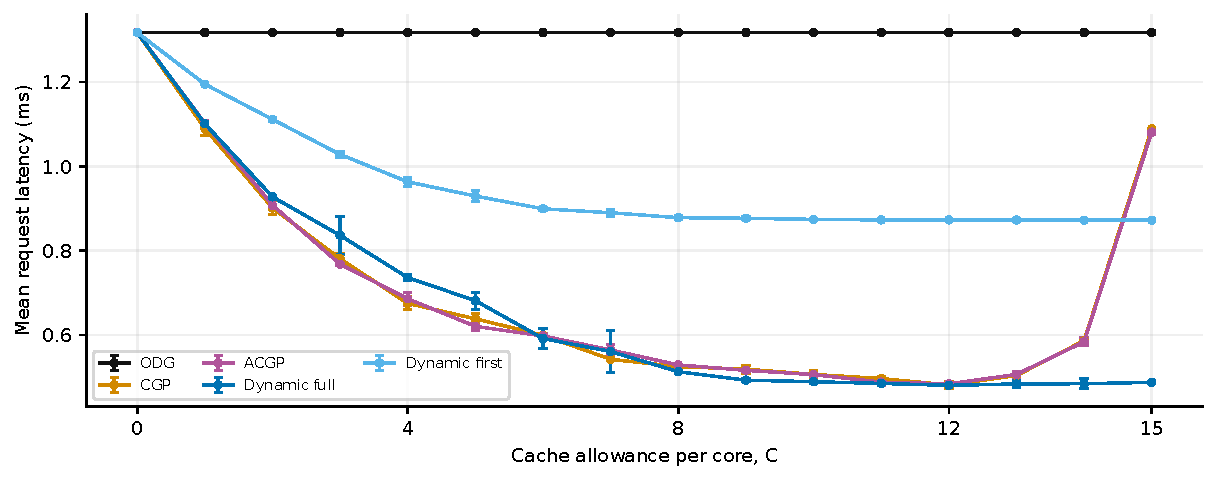
\includegraphics[width=.94\linewidth,height=.31\textheight,keepaspectratio]{figures/allocation/mesh_yx_m16.pdf}\captionof{figure}{All legal C values; ODG's C=0 result is repeated as a horizontal reference, not rerun at C>0.}\end{center}
\begin{center}{\scriptsize\setlength{\tabcolsep}{3pt}
\begin{tabular}{lrrrrr}
\toprule
C & ODG & CGP & ACGP & Dynamic full & Dynamic first \\
\midrule
0 & $1.318\pm0.000$ & $1.318\pm0.000$ & $1.318\pm0.000$ & $1.318\pm0.000$ & $1.318\pm0.000$ \\
1 & $1.318\pm0.000$ & $1.090\pm0.016$ & $1.102\pm0.007$ & $1.101\pm0.004$ & $1.195\pm0.000$ \\
2 & $1.318\pm0.000$ & $0.9019\pm0.0168$ & $0.9082\pm0.0005$ & $0.9279\pm0.0012$ & $1.112\pm0.004$ \\
3 & $1.318\pm0.000$ & $0.7810\pm0.0129$ & $0.7682\pm0.0030$ & $0.8365\pm0.0446$ & $1.029\pm0.007$ \\
4 & $1.318\pm0.000$ & $0.6753\pm0.0153$ & $0.6861\pm0.0150$ & $0.7365\pm0.0080$ & $0.9634\pm0.0113$ \\
5 & $1.318\pm0.000$ & $0.6387\pm0.0134$ & $0.6208\pm0.0107$ & $0.6816\pm0.0198$ & $0.9298\pm0.0126$ \\
6 & $1.318\pm0.000$ & $0.5997\pm0.0003$ & $0.5979\pm0.0054$ & $0.5920\pm0.0242$ & $0.8996\pm0.0037$ \\
7 & $1.318\pm0.000$ & $0.5426\pm0.0023$ & $0.5647\pm0.0131$ & $0.5610\pm0.0497$ & $0.8901\pm0.0087$ \\
8 & $1.318\pm0.000$ & $0.5252\pm0.0016$ & $0.5293\pm0.0002$ & $0.5132\pm0.0012$ & $0.8786\pm0.0048$ \\
9 & $1.318\pm0.000$ & $0.5192\pm0.0097$ & $0.5165\pm0.0026$ & $0.4932\pm0.0033$ & $0.8770\pm0.0033$ \\
10 & $1.318\pm0.000$ & $0.5067\pm0.0085$ & $0.5063\pm0.0033$ & $0.4895\pm0.0034$ & $0.8745\pm0.0009$ \\
11 & $1.318\pm0.000$ & $0.4970\pm0.0049$ & $0.4885\pm0.0069$ & $0.4854\pm0.0022$ & $0.8732\pm0.0006$ \\
12 & $1.318\pm0.000$ & $0.4817\pm0.0082$ & $0.4844\pm0.0006$ & $0.4808\pm0.0007$ & $0.8732\pm0.0002$ \\
13 & $1.318\pm0.000$ & $0.5041\pm0.0099$ & $0.5068\pm0.0062$ & $0.4842\pm0.0079$ & $0.8729\pm0.0007$ \\
14 & $1.318\pm0.000$ & $0.5869\pm0.0048$ & $0.5843\pm0.0094$ & $0.4848\pm0.0120$ & $0.8726\pm0.0011$ \\
15 & $1.318\pm0.000$ & $1.089\pm0.001$ & $1.081\pm0.005$ & $0.4880\pm0.0003$ & $0.8725\pm0.0012$ \\
\bottomrule\end{tabular}}
\captionof{table}{Mean hop latency (ms), mean $\pm$ SD. The linked CSV includes every recorded metric for every allocation.}
{\footnotesize\href{https://github.com/sanjeevkrishnaa/Compiler-Driven-ACE/blob/codex/ace-scheduler-correctness/docs/latex/qft96_final/data/allocation_mesh_yx_m16.csv}{Exact CSV values and sample counts}}
\end{center}
\clearpage\subsection*{M=32: every cache allowance}
\begin{center}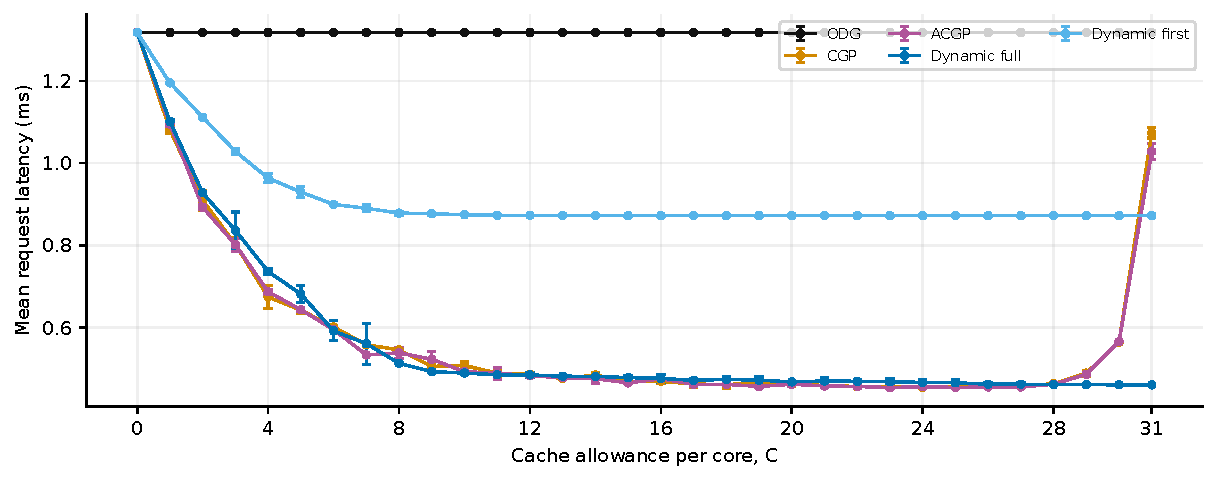
\includegraphics[width=.94\linewidth,height=.31\textheight,keepaspectratio]{figures/allocation/mesh_yx_m32.pdf}\captionof{figure}{All legal C values; ODG's C=0 result is repeated as a horizontal reference, not rerun at C>0.}\end{center}
\begin{center}{\scriptsize\setlength{\tabcolsep}{3pt}
\begin{tabular}{lrrrrr}
\toprule
C & ODG & CGP & ACGP & Dynamic full & Dynamic first \\
\midrule
0 & $1.318\pm0.000$ & $1.318\pm0.000$ & $1.318\pm0.000$ & $1.318\pm0.000$ & $1.318\pm0.000$ \\
1 & $1.318\pm0.000$ & $1.081\pm0.009$ & $1.095\pm0.007$ & $1.101\pm0.004$ & $1.195\pm0.000$ \\
2 & $1.318\pm0.000$ & $0.9092\pm0.0253$ & $0.8927\pm0.0064$ & $0.9279\pm0.0012$ & $1.112\pm0.004$ \\
3 & $1.318\pm0.000$ & $0.8024\pm0.0157$ & $0.8018\pm0.0156$ & $0.8365\pm0.0446$ & $1.029\pm0.007$ \\
4 & $1.318\pm0.000$ & $0.6744\pm0.0278$ & $0.6871\pm0.0058$ & $0.7365\pm0.0080$ & $0.9634\pm0.0113$ \\
5 & $1.318\pm0.000$ & $0.6424\pm0.0071$ & $0.6434\pm0.0044$ & $0.6816\pm0.0198$ & $0.9298\pm0.0126$ \\
6 & $1.318\pm0.000$ & $0.6016\pm0.0009$ & $0.5952\pm0.0048$ & $0.5920\pm0.0242$ & $0.8996\pm0.0037$ \\
7 & $1.318\pm0.000$ & $0.5582\pm0.0009$ & $0.5337\pm0.0010$ & $0.5610\pm0.0497$ & $0.8901\pm0.0087$ \\
8 & $1.318\pm0.000$ & $0.5457\pm0.0031$ & $0.5387\pm0.0132$ & $0.5132\pm0.0012$ & $0.8786\pm0.0048$ \\
9 & $1.318\pm0.000$ & $0.5057\pm0.0058$ & $0.5230\pm0.0200$ & $0.4932\pm0.0033$ & $0.8770\pm0.0033$ \\
10 & $1.318\pm0.000$ & $0.5079\pm0.0102$ & $0.4927\pm0.0009$ & $0.4895\pm0.0034$ & $0.8745\pm0.0009$ \\
11 & $1.318\pm0.000$ & $0.4891\pm0.0089$ & $0.4892\pm0.0147$ & $0.4853\pm0.0023$ & $0.8732\pm0.0006$ \\
12 & $1.318\pm0.000$ & $0.4861\pm0.0053$ & $0.4831\pm0.0036$ & $0.4850\pm0.0057$ & $0.8731\pm0.0001$ \\
13 & $1.318\pm0.000$ & $0.4762\pm0.0027$ & $0.4781\pm0.0005$ & $0.4819\pm0.0025$ & $0.8728\pm0.0006$ \\
14 & $1.318\pm0.000$ & $0.4845\pm0.0061$ & $0.4759\pm0.0109$ & $0.4814\pm0.0070$ & $0.8725\pm0.0009$ \\
15 & $1.318\pm0.000$ & $0.4682\pm0.0024$ & $0.4655\pm0.0005$ & $0.4785\pm0.0054$ & $0.8724\pm0.0011$ \\
16 & $1.318\pm0.000$ & $0.4695\pm0.0053$ & $0.4755\pm0.0099$ & $0.4766\pm0.0104$ & $0.8724\pm0.0011$ \\
17 & $1.318\pm0.000$ & $0.4628\pm0.0081$ & $0.4623\pm0.0065$ & $0.4718\pm0.0049$ & $0.8724\pm0.0011$ \\
18 & $1.318\pm0.000$ & $0.4613\pm0.0099$ & $0.4619\pm0.0031$ & $0.4741\pm0.0081$ & $0.8724\pm0.0011$ \\
19 & $1.318\pm0.000$ & $0.4661\pm0.0117$ & $0.4570\pm0.0022$ & $0.4722\pm0.0079$ & $0.8724\pm0.0011$ \\
20 & $1.318\pm0.000$ & $0.4619\pm0.0001$ & $0.4622\pm0.0064$ & $0.4680\pm0.0017$ & $0.8724\pm0.0011$ \\
21 & $1.318\pm0.000$ & $0.4594\pm0.0036$ & $0.4583\pm0.0026$ & $0.4702\pm0.0076$ & $0.8724\pm0.0011$ \\
22 & $1.318\pm0.000$ & $0.4567\pm0.0025$ & $0.4568\pm0.0046$ & $0.4694\pm0.0051$ & $0.8724\pm0.0011$ \\
23 & $1.318\pm0.000$ & $0.4552\pm0.0011$ & $0.4543\pm0.0028$ & $0.4687\pm0.0078$ & $0.8724\pm0.0011$ \\
24 & $1.318\pm0.000$ & $0.4548\pm0.0015$ & $0.4564\pm0.0022$ & $0.4666\pm0.0069$ & $0.8724\pm0.0011$ \\
25 & $1.318\pm0.000$ & $0.4563\pm0.0043$ & $0.4545\pm0.0030$ & $0.4658\pm0.0084$ & $0.8724\pm0.0011$ \\
26 & $1.318\pm0.000$ & $0.4571\pm0.0027$ & $0.4557\pm0.0009$ & $0.4625\pm0.0036$ & $0.8724\pm0.0011$ \\
27 & $1.318\pm0.000$ & $0.4579\pm0.0001$ & $0.4557\pm0.0015$ & $0.4624\pm0.0036$ & $0.8724\pm0.0011$ \\
28 & $1.318\pm0.000$ & $0.4634\pm0.0014$ & $0.4623\pm0.0036$ & $0.4613\pm0.0020$ & $0.8724\pm0.0011$ \\
29 & $1.318\pm0.000$ & $0.4893\pm0.0069$ & $0.4863\pm0.0033$ & $0.4613\pm0.0020$ & $0.8724\pm0.0011$ \\
30 & $1.318\pm0.000$ & $0.5648\pm0.0012$ & $0.5658\pm0.0014$ & $0.4609\pm0.0014$ & $0.8724\pm0.0011$ \\
31 & $1.318\pm0.000$ & $1.073\pm0.012$ & $1.028\pm0.019$ & $0.4607\pm0.0012$ & $0.8724\pm0.0011$ \\
\bottomrule\end{tabular}}
\captionof{table}{Mean hop latency (ms), mean $\pm$ SD. The linked CSV includes every recorded metric for every allocation.}
{\footnotesize\href{https://github.com/sanjeevkrishnaa/Compiler-Driven-ACE/blob/codex/ace-scheduler-correctness/docs/latex/qft96_final/data/allocation_mesh_yx_m32.csv}{Exact CSV values and sample counts}}
\end{center}
\section{Mesh / shortest\_reliable}
\clearpage\subsection*{M=2: every cache allowance}
\begin{center}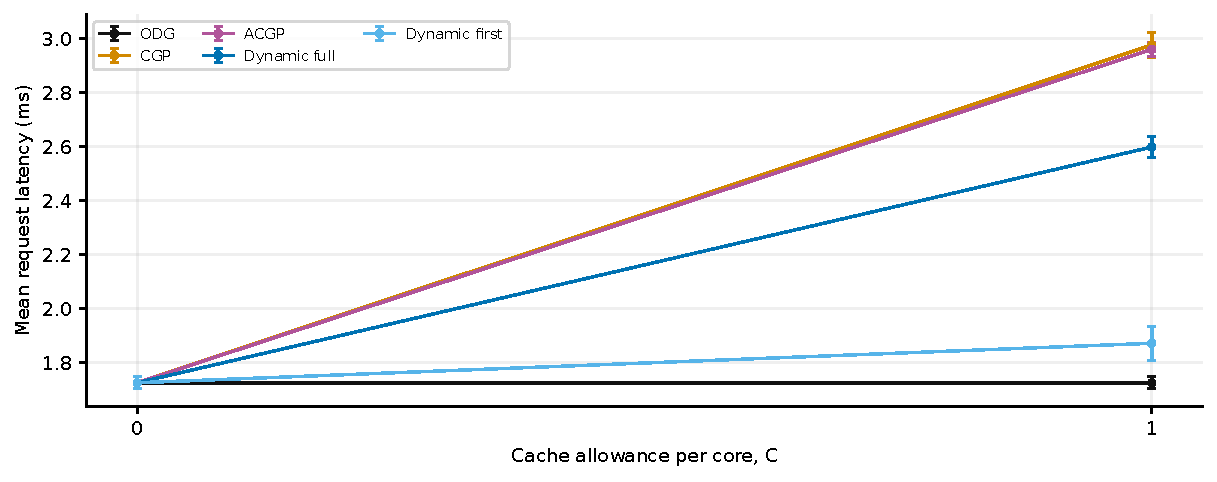
\includegraphics[width=.94\linewidth,height=.31\textheight,keepaspectratio]{figures/allocation/mesh_shortest_reliable_m2.pdf}\captionof{figure}{All legal C values; ODG's C=0 result is repeated as a horizontal reference, not rerun at C>0.}\end{center}
\begin{center}{\scriptsize\setlength{\tabcolsep}{3pt}
\begin{tabular}{lrrrrr}
\toprule
C & ODG & CGP & ACGP & Dynamic full & Dynamic first \\
\midrule
0 & $1.726\pm0.022$ & $1.726\pm0.022$ & $1.726\pm0.022$ & $1.726\pm0.022$ & $1.726\pm0.022$ \\
1 & $1.726\pm0.022$ & $2.976\pm0.047$ & $2.959\pm0.027$ & $2.598\pm0.040$ & $1.872\pm0.062$ \\
\bottomrule\end{tabular}}
\captionof{table}{Mean hop latency (ms), mean $\pm$ SD. The linked CSV includes every recorded metric for every allocation.}
{\footnotesize\href{https://github.com/sanjeevkrishnaa/Compiler-Driven-ACE/blob/codex/ace-scheduler-correctness/docs/latex/qft96_final/data/allocation_mesh_shortest_reliable_m2.csv}{Exact CSV values and sample counts}}
\end{center}
\clearpage\subsection*{M=3: every cache allowance}
\begin{center}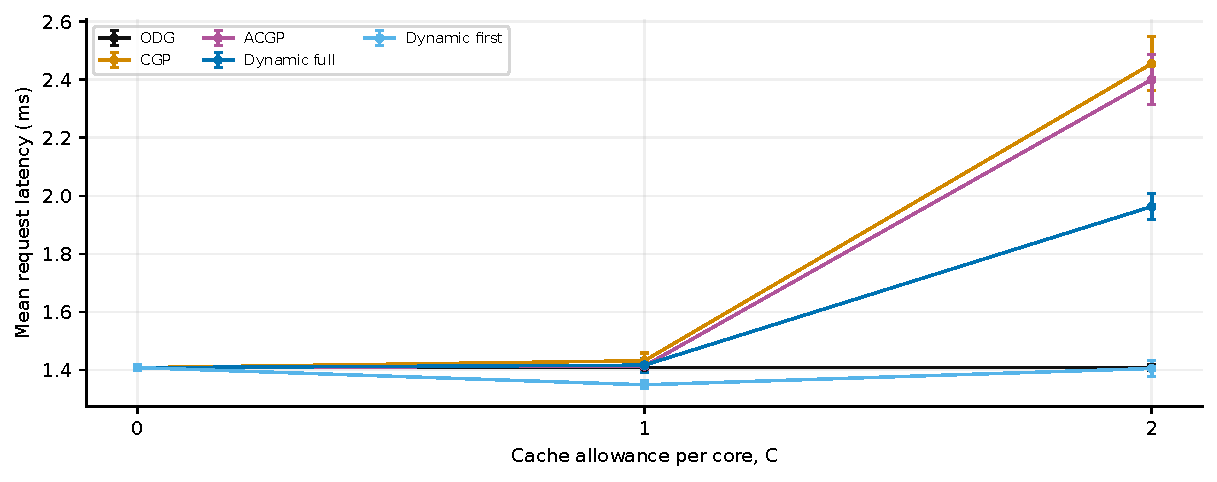
\includegraphics[width=.94\linewidth,height=.31\textheight,keepaspectratio]{figures/allocation/mesh_shortest_reliable_m3.pdf}\captionof{figure}{All legal C values; ODG's C=0 result is repeated as a horizontal reference, not rerun at C>0.}\end{center}
\begin{center}{\scriptsize\setlength{\tabcolsep}{3pt}
\begin{tabular}{lrrrrr}
\toprule
C & ODG & CGP & ACGP & Dynamic full & Dynamic first \\
\midrule
0 & $1.408\pm0.010$ & $1.408\pm0.010$ & $1.408\pm0.010$ & $1.408\pm0.010$ & $1.408\pm0.010$ \\
1 & $1.408\pm0.010$ & $1.432\pm0.027$ & $1.414\pm0.012$ & $1.417\pm0.024$ & $1.349\pm0.014$ \\
2 & $1.408\pm0.010$ & $2.455\pm0.093$ & $2.401\pm0.085$ & $1.963\pm0.046$ & $1.405\pm0.028$ \\
\bottomrule\end{tabular}}
\captionof{table}{Mean hop latency (ms), mean $\pm$ SD. The linked CSV includes every recorded metric for every allocation.}
{\footnotesize\href{https://github.com/sanjeevkrishnaa/Compiler-Driven-ACE/blob/codex/ace-scheduler-correctness/docs/latex/qft96_final/data/allocation_mesh_shortest_reliable_m3.csv}{Exact CSV values and sample counts}}
\end{center}
\clearpage\subsection*{M=4: every cache allowance}
\begin{center}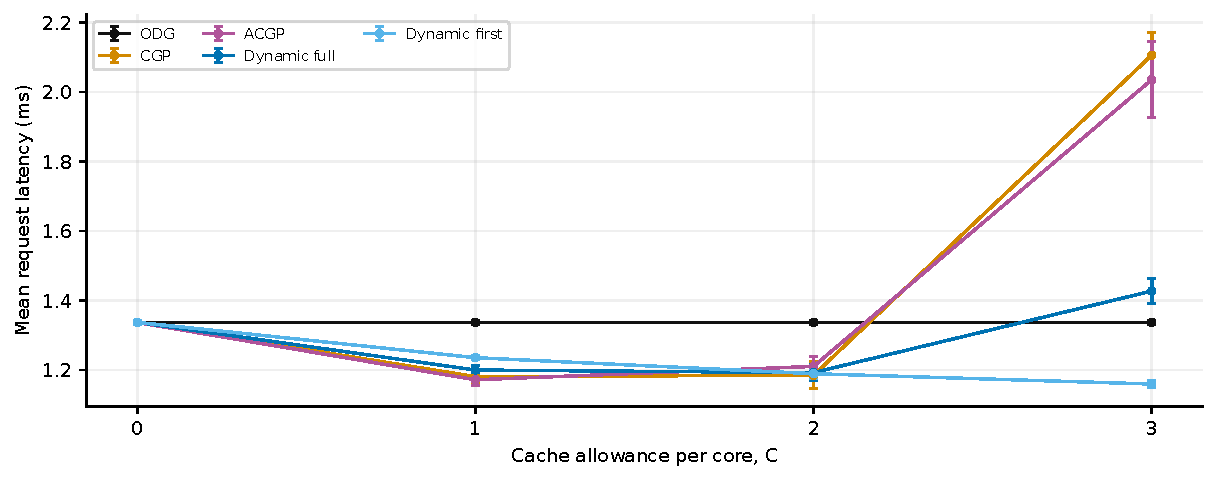
\includegraphics[width=.94\linewidth,height=.31\textheight,keepaspectratio]{figures/allocation/mesh_shortest_reliable_m4.pdf}\captionof{figure}{All legal C values; ODG's C=0 result is repeated as a horizontal reference, not rerun at C>0.}\end{center}
\begin{center}{\scriptsize\setlength{\tabcolsep}{3pt}
\begin{tabular}{lrrrrr}
\toprule
C & ODG & CGP & ACGP & Dynamic full & Dynamic first \\
\midrule
0 & $1.337\pm0.005$ & $1.337\pm0.005$ & $1.337\pm0.005$ & $1.337\pm0.005$ & $1.337\pm0.005$ \\
1 & $1.337\pm0.005$ & $1.181\pm0.019$ & $1.172\pm0.016$ & $1.200\pm0.014$ & $1.235\pm0.005$ \\
2 & $1.337\pm0.005$ & $1.185\pm0.039$ & $1.210\pm0.030$ & $1.192\pm0.022$ & $1.189\pm0.013$ \\
3 & $1.337\pm0.005$ & $2.106\pm0.066$ & $2.035\pm0.109$ & $1.427\pm0.036$ & $1.160\pm0.010$ \\
\bottomrule\end{tabular}}
\captionof{table}{Mean hop latency (ms), mean $\pm$ SD. The linked CSV includes every recorded metric for every allocation.}
{\footnotesize\href{https://github.com/sanjeevkrishnaa/Compiler-Driven-ACE/blob/codex/ace-scheduler-correctness/docs/latex/qft96_final/data/allocation_mesh_shortest_reliable_m4.csv}{Exact CSV values and sample counts}}
\end{center}
\clearpage\subsection*{M=6: every cache allowance}
\begin{center}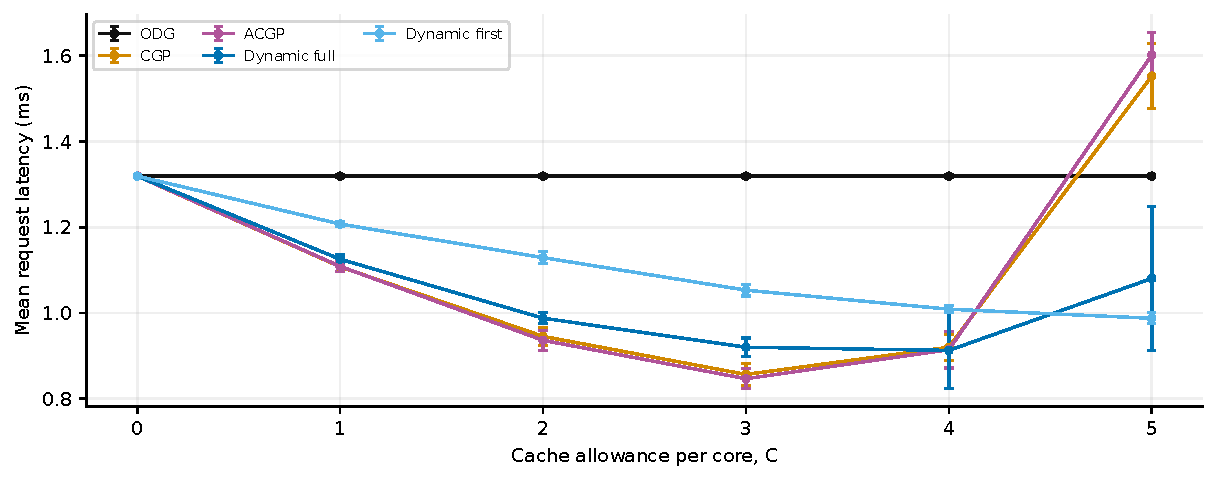
\includegraphics[width=.94\linewidth,height=.31\textheight,keepaspectratio]{figures/allocation/mesh_shortest_reliable_m6.pdf}\captionof{figure}{All legal C values; ODG's C=0 result is repeated as a horizontal reference, not rerun at C>0.}\end{center}
\begin{center}{\scriptsize\setlength{\tabcolsep}{3pt}
\begin{tabular}{lrrrrr}
\toprule
C & ODG & CGP & ACGP & Dynamic full & Dynamic first \\
\midrule
0 & $1.319\pm0.004$ & $1.319\pm0.004$ & $1.319\pm0.004$ & $1.319\pm0.004$ & $1.319\pm0.004$ \\
1 & $1.319\pm0.004$ & $1.108\pm0.012$ & $1.109\pm0.013$ & $1.125\pm0.010$ & $1.207\pm0.006$ \\
2 & $1.319\pm0.004$ & $0.9452\pm0.0212$ & $0.9362\pm0.0231$ & $0.9878\pm0.0124$ & $1.129\pm0.015$ \\
3 & $1.319\pm0.004$ & $0.8564\pm0.0263$ & $0.8465\pm0.0234$ & $0.9199\pm0.0217$ & $1.053\pm0.014$ \\
4 & $1.319\pm0.004$ & $0.9200\pm0.0303$ & $0.9142\pm0.0427$ & $0.9125\pm0.0893$ & $1.009\pm0.008$ \\
5 & $1.319\pm0.004$ & $1.553\pm0.077$ & $1.602\pm0.053$ & $1.080\pm0.169$ & $0.9875\pm0.0125$ \\
\bottomrule\end{tabular}}
\captionof{table}{Mean hop latency (ms), mean $\pm$ SD. The linked CSV includes every recorded metric for every allocation.}
{\footnotesize\href{https://github.com/sanjeevkrishnaa/Compiler-Driven-ACE/blob/codex/ace-scheduler-correctness/docs/latex/qft96_final/data/allocation_mesh_shortest_reliable_m6.csv}{Exact CSV values and sample counts}}
\end{center}
\clearpage\subsection*{M=8: every cache allowance}
\begin{center}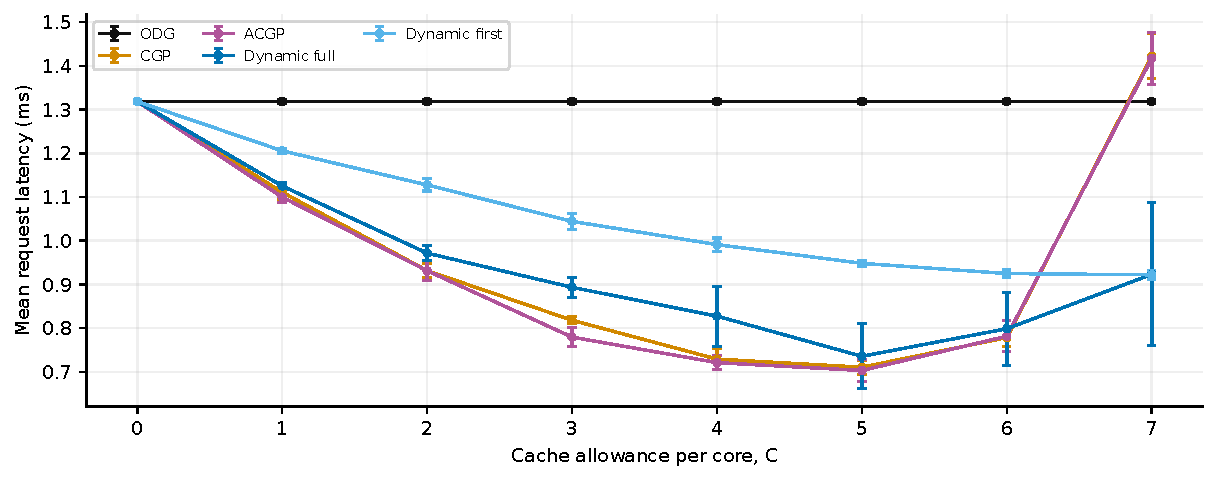
\includegraphics[width=.94\linewidth,height=.31\textheight,keepaspectratio]{figures/allocation/mesh_shortest_reliable_m8.pdf}\captionof{figure}{All legal C values; ODG's C=0 result is repeated as a horizontal reference, not rerun at C>0.}\end{center}
\begin{center}{\scriptsize\setlength{\tabcolsep}{3pt}
\begin{tabular}{lrrrrr}
\toprule
C & ODG & CGP & ACGP & Dynamic full & Dynamic first \\
\midrule
0 & $1.319\pm0.004$ & $1.319\pm0.004$ & $1.319\pm0.004$ & $1.319\pm0.004$ & $1.319\pm0.004$ \\
1 & $1.319\pm0.004$ & $1.111\pm0.017$ & $1.100\pm0.012$ & $1.125\pm0.008$ & $1.206\pm0.006$ \\
2 & $1.319\pm0.004$ & $0.9315\pm0.0164$ & $0.9314\pm0.0229$ & $0.9716\pm0.0166$ & $1.128\pm0.014$ \\
3 & $1.319\pm0.004$ & $0.8181\pm0.0076$ & $0.7795\pm0.0224$ & $0.8935\pm0.0224$ & $1.044\pm0.018$ \\
4 & $1.319\pm0.004$ & $0.7292\pm0.0236$ & $0.7211\pm0.0157$ & $0.8275\pm0.0688$ & $0.9912\pm0.0150$ \\
5 & $1.319\pm0.004$ & $0.7106\pm0.0165$ & $0.7031\pm0.0258$ & $0.7356\pm0.0742$ & $0.9483\pm0.0074$ \\
6 & $1.319\pm0.004$ & $0.7786\pm0.0201$ & $0.7816\pm0.0353$ & $0.7988\pm0.0835$ & $0.9249\pm0.0088$ \\
7 & $1.319\pm0.004$ & $1.422\pm0.051$ & $1.417\pm0.059$ & $0.9230\pm0.1635$ & $0.9220\pm0.0102$ \\
\bottomrule\end{tabular}}
\captionof{table}{Mean hop latency (ms), mean $\pm$ SD. The linked CSV includes every recorded metric for every allocation.}
{\footnotesize\href{https://github.com/sanjeevkrishnaa/Compiler-Driven-ACE/blob/codex/ace-scheduler-correctness/docs/latex/qft96_final/data/allocation_mesh_shortest_reliable_m8.csv}{Exact CSV values and sample counts}}
\end{center}
\clearpage\subsection*{M=16: every cache allowance}
\begin{center}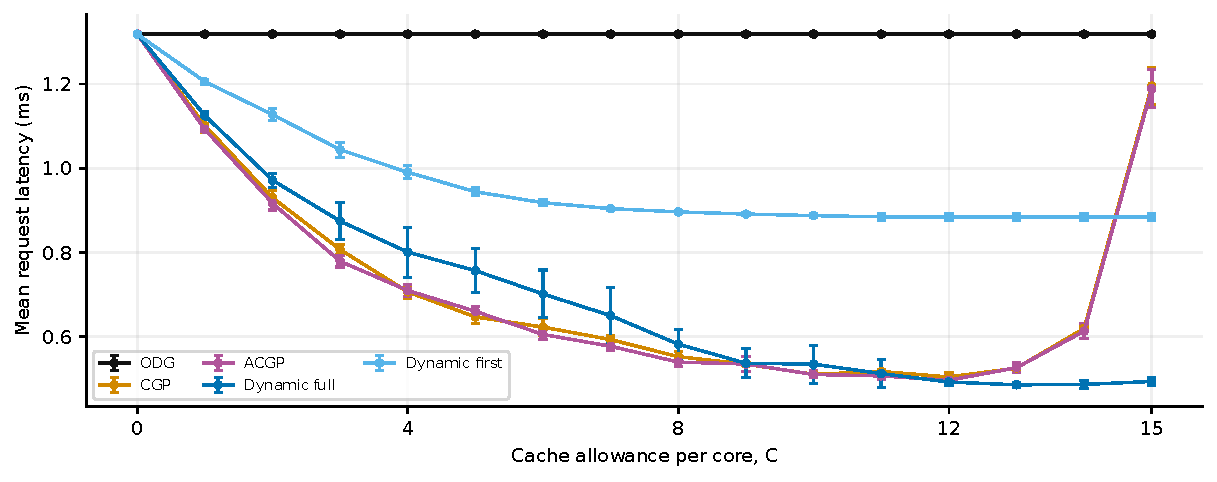
\includegraphics[width=.94\linewidth,height=.31\textheight,keepaspectratio]{figures/allocation/mesh_shortest_reliable_m16.pdf}\captionof{figure}{All legal C values; ODG's C=0 result is repeated as a horizontal reference, not rerun at C>0.}\end{center}
\begin{center}{\scriptsize\setlength{\tabcolsep}{3pt}
\begin{tabular}{lrrrrr}
\toprule
C & ODG & CGP & ACGP & Dynamic full & Dynamic first \\
\midrule
0 & $1.318\pm0.004$ & $1.319\pm0.004$ & $1.319\pm0.004$ & $1.318\pm0.004$ & $1.318\pm0.004$ \\
1 & $1.318\pm0.004$ & $1.101\pm0.016$ & $1.093\pm0.006$ & $1.125\pm0.008$ & $1.206\pm0.006$ \\
2 & $1.318\pm0.004$ & $0.9303\pm0.0161$ & $0.9171\pm0.0160$ & $0.9718\pm0.0167$ & $1.128\pm0.014$ \\
3 & $1.318\pm0.004$ & $0.8072\pm0.0116$ & $0.7793\pm0.0137$ & $0.8746\pm0.0438$ & $1.044\pm0.018$ \\
4 & $1.318\pm0.004$ & $0.7066\pm0.0145$ & $0.7099\pm0.0151$ & $0.8011\pm0.0592$ & $0.9906\pm0.0152$ \\
5 & $1.318\pm0.004$ & $0.6472\pm0.0159$ & $0.6604\pm0.0124$ & $0.7570\pm0.0520$ & $0.9444\pm0.0096$ \\
6 & $1.318\pm0.004$ & $0.6230\pm0.0207$ & $0.6056\pm0.0127$ & $0.7017\pm0.0568$ & $0.9184\pm0.0077$ \\
7 & $1.318\pm0.004$ & $0.5934\pm0.0089$ & $0.5776\pm0.0107$ & $0.6502\pm0.0659$ & $0.9043\pm0.0037$ \\
8 & $1.318\pm0.004$ & $0.5529\pm0.0116$ & $0.5400\pm0.0094$ & $0.5825\pm0.0358$ & $0.8965\pm0.0027$ \\
9 & $1.318\pm0.004$ & $0.5350\pm0.0038$ & $0.5355\pm0.0178$ & $0.5372\pm0.0348$ & $0.8914\pm0.0042$ \\
10 & $1.318\pm0.004$ & $0.5110\pm0.0057$ & $0.5106\pm0.0082$ & $0.5351\pm0.0453$ & $0.8877\pm0.0040$ \\
11 & $1.318\pm0.004$ & $0.5177\pm0.0035$ & $0.5072\pm0.0096$ & $0.5127\pm0.0331$ & $0.8848\pm0.0079$ \\
12 & $1.318\pm0.004$ & $0.5047\pm0.0098$ & $0.4969\pm0.0108$ & $0.4927\pm0.0088$ & $0.8843\pm0.0084$ \\
13 & $1.318\pm0.004$ & $0.5257\pm0.0109$ & $0.5268\pm0.0111$ & $0.4860\pm0.0065$ & $0.8841\pm0.0083$ \\
14 & $1.318\pm0.004$ & $0.6198\pm0.0058$ & $0.6135\pm0.0183$ & $0.4869\pm0.0102$ & $0.8841\pm0.0083$ \\
15 & $1.318\pm0.004$ & $1.195\pm0.043$ & $1.189\pm0.046$ & $0.4941\pm0.0101$ & $0.8841\pm0.0083$ \\
\bottomrule\end{tabular}}
\captionof{table}{Mean hop latency (ms), mean $\pm$ SD. The linked CSV includes every recorded metric for every allocation.}
{\footnotesize\href{https://github.com/sanjeevkrishnaa/Compiler-Driven-ACE/blob/codex/ace-scheduler-correctness/docs/latex/qft96_final/data/allocation_mesh_shortest_reliable_m16.csv}{Exact CSV values and sample counts}}
\end{center}
\clearpage\subsection*{M=32: every cache allowance}
\begin{center}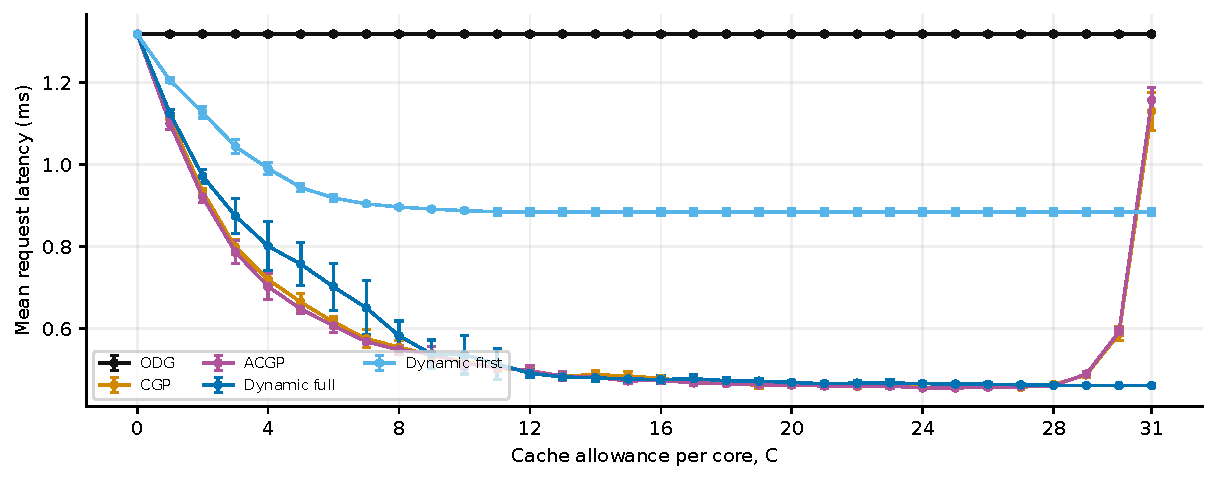
\includegraphics[width=.94\linewidth,height=.31\textheight,keepaspectratio]{figures/allocation/mesh_shortest_reliable_m32.pdf}\captionof{figure}{All legal C values; ODG's C=0 result is repeated as a horizontal reference, not rerun at C>0.}\end{center}
\begin{center}{\scriptsize\setlength{\tabcolsep}{3pt}
\begin{tabular}{lrrrrr}
\toprule
C & ODG & CGP & ACGP & Dynamic full & Dynamic first \\
\midrule
0 & $1.318\pm0.004$ & $1.319\pm0.004$ & $1.319\pm0.004$ & $1.318\pm0.004$ & $1.318\pm0.004$ \\
1 & $1.318\pm0.004$ & $1.112\pm0.011$ & $1.101\pm0.015$ & $1.125\pm0.008$ & $1.206\pm0.006$ \\
2 & $1.318\pm0.004$ & $0.9347\pm0.0073$ & $0.9211\pm0.0127$ & $0.9718\pm0.0167$ & $1.128\pm0.014$ \\
3 & $1.318\pm0.004$ & $0.7987\pm0.0176$ & $0.7865\pm0.0272$ & $0.8746\pm0.0438$ & $1.044\pm0.018$ \\
4 & $1.318\pm0.004$ & $0.7198\pm0.0203$ & $0.7025\pm0.0325$ & $0.8011\pm0.0592$ & $0.9906\pm0.0152$ \\
5 & $1.318\pm0.004$ & $0.6642\pm0.0218$ & $0.6474\pm0.0104$ & $0.7570\pm0.0520$ & $0.9444\pm0.0096$ \\
6 & $1.318\pm0.004$ & $0.6155\pm0.0140$ & $0.6063\pm0.0166$ & $0.7017\pm0.0568$ & $0.9184\pm0.0077$ \\
7 & $1.318\pm0.004$ & $0.5755\pm0.0210$ & $0.5679\pm0.0053$ & $0.6502\pm0.0659$ & $0.9043\pm0.0037$ \\
8 & $1.318\pm0.004$ & $0.5543\pm0.0170$ & $0.5481\pm0.0107$ & $0.5825\pm0.0358$ & $0.8965\pm0.0027$ \\
9 & $1.318\pm0.004$ & $0.5342\pm0.0094$ & $0.5383\pm0.0177$ & $0.5372\pm0.0348$ & $0.8914\pm0.0042$ \\
10 & $1.318\pm0.004$ & $0.5201\pm0.0131$ & $0.5141\pm0.0142$ & $0.5356\pm0.0467$ & $0.8877\pm0.0040$ \\
11 & $1.318\pm0.004$ & $0.5035\pm0.0086$ & $0.5064\pm0.0058$ & $0.5134\pm0.0370$ & $0.8848\pm0.0079$ \\
12 & $1.318\pm0.004$ & $0.4971\pm0.0080$ & $0.4964\pm0.0126$ & $0.4906\pm0.0092$ & $0.8843\pm0.0084$ \\
13 & $1.318\pm0.004$ & $0.4840\pm0.0064$ & $0.4838\pm0.0104$ & $0.4818\pm0.0060$ & $0.8841\pm0.0083$ \\
14 & $1.318\pm0.004$ & $0.4873\pm0.0112$ & $0.4808\pm0.0105$ & $0.4796\pm0.0091$ & $0.8841\pm0.0083$ \\
15 & $1.318\pm0.004$ & $0.4841\pm0.0100$ & $0.4722\pm0.0059$ & $0.4768\pm0.0081$ & $0.8841\pm0.0083$ \\
16 & $1.318\pm0.004$ & $0.4784\pm0.0058$ & $0.4735\pm0.0082$ & $0.4755\pm0.0103$ & $0.8841\pm0.0083$ \\
17 & $1.318\pm0.004$ & $0.4691\pm0.0061$ & $0.4674\pm0.0055$ & $0.4775\pm0.0101$ & $0.8841\pm0.0083$ \\
18 & $1.318\pm0.004$ & $0.4656\pm0.0045$ & $0.4653\pm0.0033$ & $0.4727\pm0.0069$ & $0.8841\pm0.0083$ \\
19 & $1.318\pm0.004$ & $0.4617\pm0.0068$ & $0.4625\pm0.0049$ & $0.4717\pm0.0072$ & $0.8841\pm0.0083$ \\
20 & $1.318\pm0.004$ & $0.4626\pm0.0060$ & $0.4621\pm0.0045$ & $0.4684\pm0.0046$ & $0.8841\pm0.0083$ \\
21 & $1.318\pm0.004$ & $0.4600\pm0.0070$ & $0.4599\pm0.0069$ & $0.4653\pm0.0045$ & $0.8841\pm0.0083$ \\
22 & $1.318\pm0.004$ & $0.4589\pm0.0043$ & $0.4599\pm0.0043$ & $0.4668\pm0.0062$ & $0.8841\pm0.0083$ \\
23 & $1.318\pm0.004$ & $0.4595\pm0.0049$ & $0.4597\pm0.0055$ & $0.4673\pm0.0072$ & $0.8841\pm0.0083$ \\
24 & $1.318\pm0.004$ & $0.4562\pm0.0020$ & $0.4548\pm0.0009$ & $0.4654\pm0.0053$ & $0.8841\pm0.0083$ \\
25 & $1.318\pm0.004$ & $0.4581\pm0.0037$ & $0.4550\pm0.0011$ & $0.4646\pm0.0043$ & $0.8841\pm0.0083$ \\
26 & $1.318\pm0.004$ & $0.4592\pm0.0042$ & $0.4567\pm0.0026$ & $0.4639\pm0.0042$ & $0.8841\pm0.0083$ \\
27 & $1.318\pm0.004$ & $0.4565\pm0.0014$ & $0.4581\pm0.0026$ & $0.4625\pm0.0028$ & $0.8841\pm0.0083$ \\
28 & $1.318\pm0.004$ & $0.4632\pm0.0018$ & $0.4607\pm0.0030$ & $0.4617\pm0.0025$ & $0.8841\pm0.0083$ \\
29 & $1.318\pm0.004$ & $0.4868\pm0.0064$ & $0.4887\pm0.0068$ & $0.4610\pm0.0014$ & $0.8841\pm0.0083$ \\
30 & $1.318\pm0.004$ & $0.5873\pm0.0176$ & $0.5921\pm0.0092$ & $0.4607\pm0.0011$ & $0.8841\pm0.0083$ \\
31 & $1.318\pm0.004$ & $1.130\pm0.046$ & $1.157\pm0.030$ & $0.4607\pm0.0011$ & $0.8841\pm0.0083$ \\
\bottomrule\end{tabular}}
\captionof{table}{Mean hop latency (ms), mean $\pm$ SD. The linked CSV includes every recorded metric for every allocation.}
{\footnotesize\href{https://github.com/sanjeevkrishnaa/Compiler-Driven-ACE/blob/codex/ace-scheduler-correctness/docs/latex/qft96_final/data/allocation_mesh_shortest_reliable_m32.csv}{Exact CSV values and sample counts}}
\end{center}
\section{Mesh / max\_reliability}
\clearpage\subsection*{M=2: every cache allowance}
\begin{center}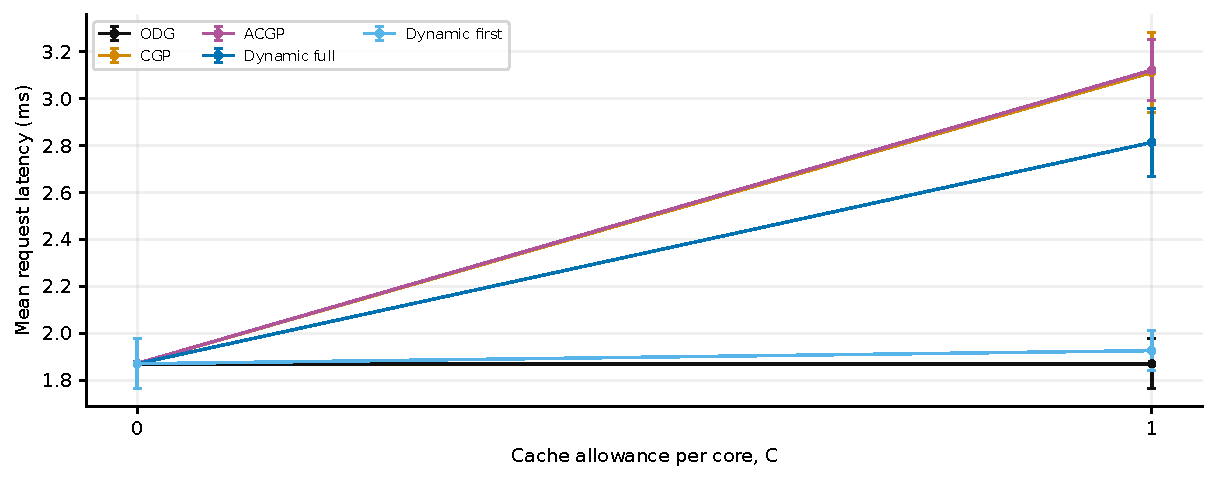
\includegraphics[width=.94\linewidth,height=.31\textheight,keepaspectratio]{figures/allocation/mesh_max_reliability_m2.pdf}\captionof{figure}{All legal C values; ODG's C=0 result is repeated as a horizontal reference, not rerun at C>0.}\end{center}
\begin{center}{\scriptsize\setlength{\tabcolsep}{3pt}
\begin{tabular}{lrrrrr}
\toprule
C & ODG & CGP & ACGP & Dynamic full & Dynamic first \\
\midrule
0 & $1.871\pm0.106$ & $1.872\pm0.107$ & $1.872\pm0.107$ & $1.871\pm0.106$ & $1.871\pm0.106$ \\
1 & $1.871\pm0.106$ & $3.111\pm0.170$ & $3.120\pm0.130$ & $2.813\pm0.145$ & $1.926\pm0.084$ \\
\bottomrule\end{tabular}}
\captionof{table}{Mean hop latency (ms), mean $\pm$ SD. The linked CSV includes every recorded metric for every allocation.}
{\footnotesize\href{https://github.com/sanjeevkrishnaa/Compiler-Driven-ACE/blob/codex/ace-scheduler-correctness/docs/latex/qft96_final/data/allocation_mesh_max_reliability_m2.csv}{Exact CSV values and sample counts}}
\end{center}
\clearpage\subsection*{M=3: every cache allowance}
\begin{center}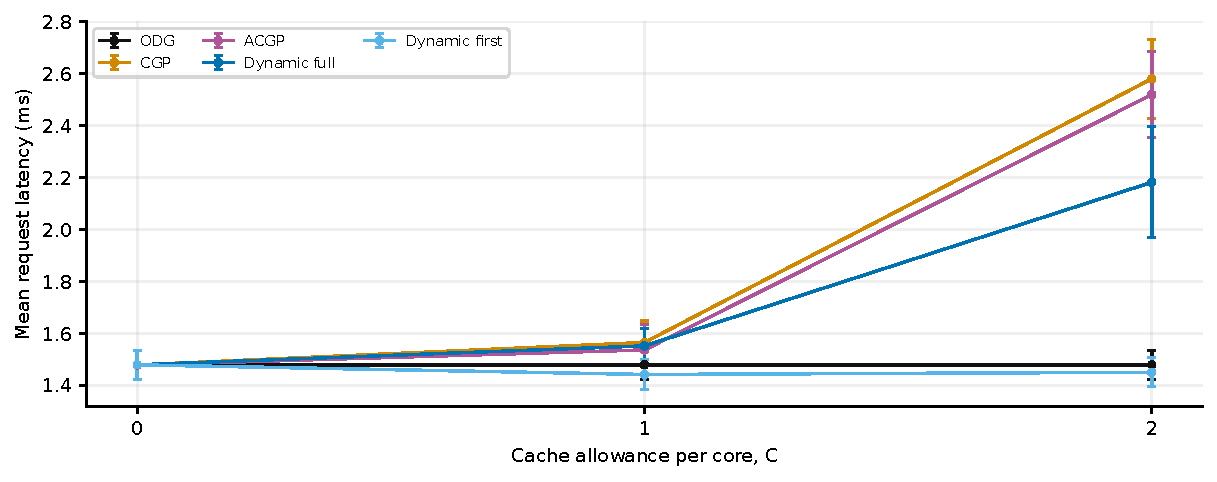
\includegraphics[width=.94\linewidth,height=.31\textheight,keepaspectratio]{figures/allocation/mesh_max_reliability_m3.pdf}\captionof{figure}{All legal C values; ODG's C=0 result is repeated as a horizontal reference, not rerun at C>0.}\end{center}
\begin{center}{\scriptsize\setlength{\tabcolsep}{3pt}
\begin{tabular}{lrrrrr}
\toprule
C & ODG & CGP & ACGP & Dynamic full & Dynamic first \\
\midrule
0 & $1.479\pm0.057$ & $1.479\pm0.056$ & $1.479\pm0.056$ & $1.479\pm0.057$ & $1.479\pm0.057$ \\
1 & $1.479\pm0.057$ & $1.565\pm0.083$ & $1.536\pm0.097$ & $1.552\pm0.068$ & $1.442\pm0.056$ \\
2 & $1.479\pm0.057$ & $2.580\pm0.153$ & $2.519\pm0.165$ & $2.182\pm0.213$ & $1.450\pm0.056$ \\
\bottomrule\end{tabular}}
\captionof{table}{Mean hop latency (ms), mean $\pm$ SD. The linked CSV includes every recorded metric for every allocation.}
{\footnotesize\href{https://github.com/sanjeevkrishnaa/Compiler-Driven-ACE/blob/codex/ace-scheduler-correctness/docs/latex/qft96_final/data/allocation_mesh_max_reliability_m3.csv}{Exact CSV values and sample counts}}
\end{center}
\clearpage\subsection*{M=4: every cache allowance}
\begin{center}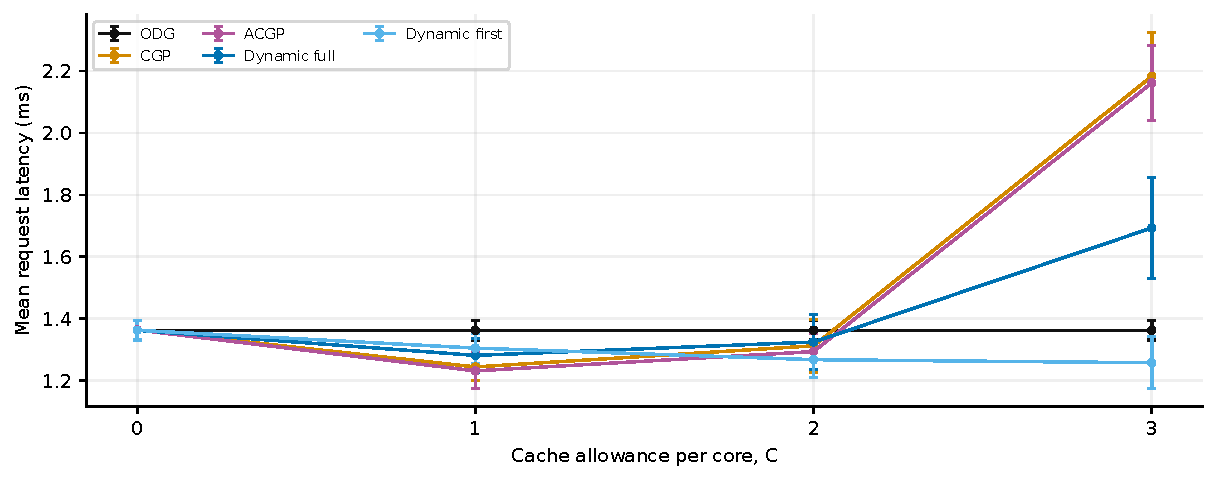
\includegraphics[width=.94\linewidth,height=.31\textheight,keepaspectratio]{figures/allocation/mesh_max_reliability_m4.pdf}\captionof{figure}{All legal C values; ODG's C=0 result is repeated as a horizontal reference, not rerun at C>0.}\end{center}
\begin{center}{\scriptsize\setlength{\tabcolsep}{3pt}
\begin{tabular}{lrrrrr}
\toprule
C & ODG & CGP & ACGP & Dynamic full & Dynamic first \\
\midrule
0 & $1.362\pm0.032$ & $1.363\pm0.032$ & $1.363\pm0.032$ & $1.362\pm0.032$ & $1.362\pm0.032$ \\
1 & $1.362\pm0.032$ & $1.244\pm0.045$ & $1.231\pm0.058$ & $1.281\pm0.054$ & $1.305\pm0.048$ \\
2 & $1.362\pm0.032$ & $1.312\pm0.085$ & $1.293\pm0.058$ & $1.324\pm0.089$ & $1.267\pm0.058$ \\
3 & $1.362\pm0.032$ & $2.183\pm0.142$ & $2.162\pm0.120$ & $1.693\pm0.164$ & $1.257\pm0.083$ \\
\bottomrule\end{tabular}}
\captionof{table}{Mean hop latency (ms), mean $\pm$ SD. The linked CSV includes every recorded metric for every allocation.}
{\footnotesize\href{https://github.com/sanjeevkrishnaa/Compiler-Driven-ACE/blob/codex/ace-scheduler-correctness/docs/latex/qft96_final/data/allocation_mesh_max_reliability_m4.csv}{Exact CSV values and sample counts}}
\end{center}
\clearpage\subsection*{M=6: every cache allowance}
\begin{center}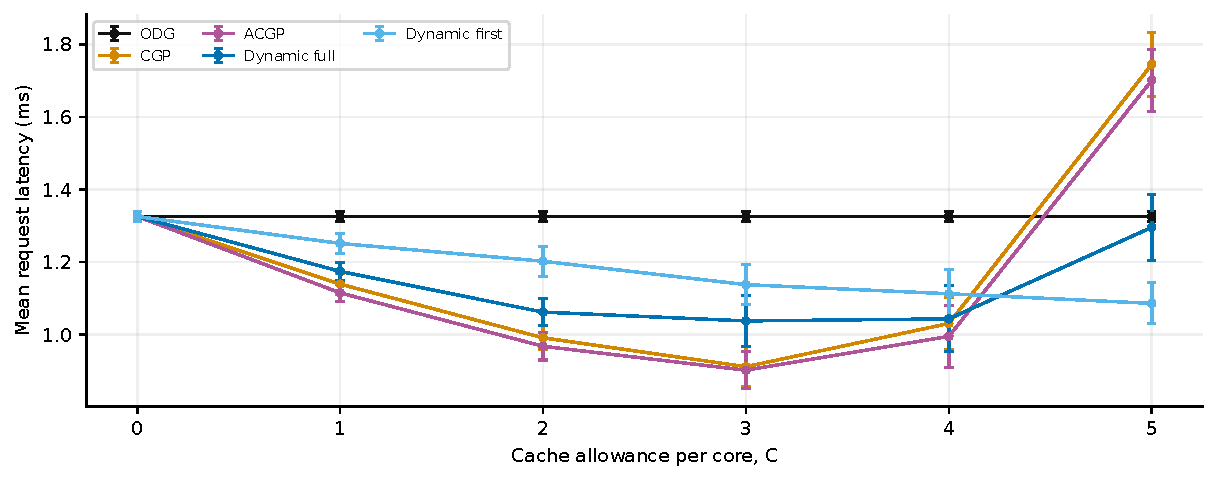
\includegraphics[width=.94\linewidth,height=.31\textheight,keepaspectratio]{figures/allocation/mesh_max_reliability_m6.pdf}\captionof{figure}{All legal C values; ODG's C=0 result is repeated as a horizontal reference, not rerun at C>0.}\end{center}
\begin{center}{\scriptsize\setlength{\tabcolsep}{3pt}
\begin{tabular}{lrrrrr}
\toprule
C & ODG & CGP & ACGP & Dynamic full & Dynamic first \\
\midrule
0 & $1.326\pm0.014$ & $1.326\pm0.014$ & $1.326\pm0.014$ & $1.326\pm0.014$ & $1.326\pm0.014$ \\
1 & $1.326\pm0.014$ & $1.140\pm0.028$ & $1.115\pm0.024$ & $1.175\pm0.024$ & $1.252\pm0.027$ \\
2 & $1.326\pm0.014$ & $0.9917\pm0.0332$ & $0.9684\pm0.0378$ & $1.062\pm0.038$ & $1.203\pm0.042$ \\
3 & $1.326\pm0.014$ & $0.9121\pm0.0551$ & $0.9024\pm0.0510$ & $1.038\pm0.071$ & $1.138\pm0.055$ \\
4 & $1.326\pm0.014$ & $1.031\pm0.073$ & $0.9958\pm0.0857$ & $1.044\pm0.091$ & $1.113\pm0.067$ \\
5 & $1.326\pm0.014$ & $1.745\pm0.088$ & $1.701\pm0.085$ & $1.296\pm0.090$ & $1.086\pm0.056$ \\
\bottomrule\end{tabular}}
\captionof{table}{Mean hop latency (ms), mean $\pm$ SD. The linked CSV includes every recorded metric for every allocation.}
{\footnotesize\href{https://github.com/sanjeevkrishnaa/Compiler-Driven-ACE/blob/codex/ace-scheduler-correctness/docs/latex/qft96_final/data/allocation_mesh_max_reliability_m6.csv}{Exact CSV values and sample counts}}
\end{center}
\clearpage\subsection*{M=8: every cache allowance}
\begin{center}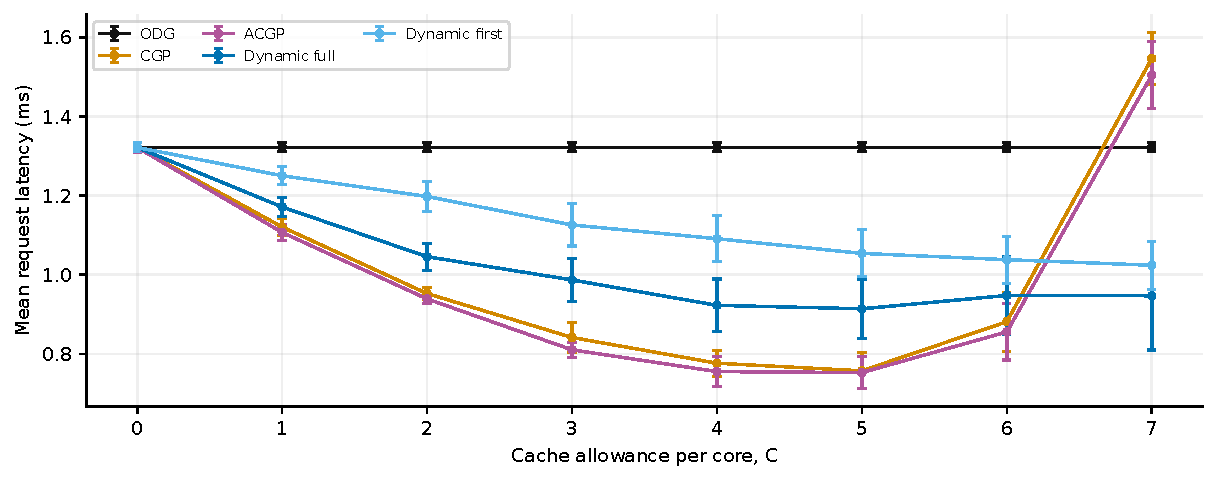
\includegraphics[width=.94\linewidth,height=.31\textheight,keepaspectratio]{figures/allocation/mesh_max_reliability_m8.pdf}\captionof{figure}{All legal C values; ODG's C=0 result is repeated as a horizontal reference, not rerun at C>0.}\end{center}
\begin{center}{\scriptsize\setlength{\tabcolsep}{3pt}
\begin{tabular}{lrrrrr}
\toprule
C & ODG & CGP & ACGP & Dynamic full & Dynamic first \\
\midrule
0 & $1.322\pm0.011$ & $1.322\pm0.011$ & $1.322\pm0.011$ & $1.322\pm0.011$ & $1.322\pm0.011$ \\
1 & $1.322\pm0.011$ & $1.121\pm0.021$ & $1.107\pm0.020$ & $1.171\pm0.025$ & $1.250\pm0.022$ \\
2 & $1.322\pm0.011$ & $0.9525\pm0.0153$ & $0.9390\pm0.0126$ & $1.046\pm0.034$ & $1.198\pm0.039$ \\
3 & $1.322\pm0.011$ & $0.8416\pm0.0375$ & $0.8104\pm0.0195$ & $0.9869\pm0.0548$ & $1.126\pm0.053$ \\
4 & $1.322\pm0.011$ & $0.7766\pm0.0332$ & $0.7554\pm0.0378$ & $0.9228\pm0.0665$ & $1.091\pm0.058$ \\
5 & $1.322\pm0.011$ & $0.7573\pm0.0452$ & $0.7530\pm0.0399$ & $0.9140\pm0.0743$ & $1.054\pm0.059$ \\
6 & $1.322\pm0.011$ & $0.8815\pm0.0746$ & $0.8556\pm0.0710$ & $0.9477\pm0.0990$ & $1.038\pm0.059$ \\
7 & $1.322\pm0.011$ & $1.546\pm0.066$ & $1.504\pm0.085$ & $0.9469\pm0.1370$ & $1.024\pm0.061$ \\
\bottomrule\end{tabular}}
\captionof{table}{Mean hop latency (ms), mean $\pm$ SD. The linked CSV includes every recorded metric for every allocation.}
{\footnotesize\href{https://github.com/sanjeevkrishnaa/Compiler-Driven-ACE/blob/codex/ace-scheduler-correctness/docs/latex/qft96_final/data/allocation_mesh_max_reliability_m8.csv}{Exact CSV values and sample counts}}
\end{center}
\clearpage\subsection*{M=16: every cache allowance}
\begin{center}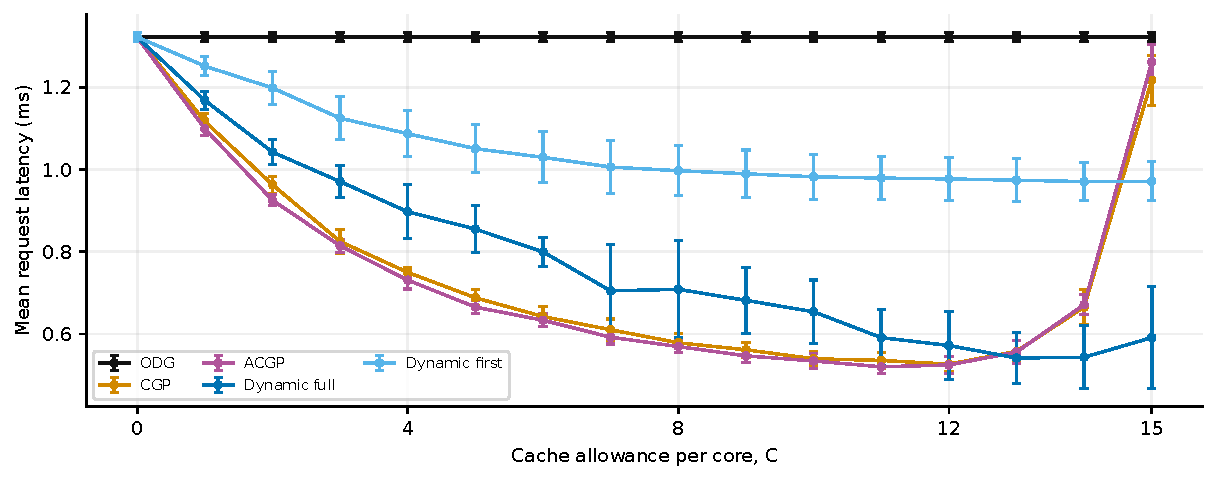
\includegraphics[width=.94\linewidth,height=.31\textheight,keepaspectratio]{figures/allocation/mesh_max_reliability_m16.pdf}\captionof{figure}{All legal C values; ODG's C=0 result is repeated as a horizontal reference, not rerun at C>0.}\end{center}
\begin{center}{\scriptsize\setlength{\tabcolsep}{3pt}
\begin{tabular}{lrrrrr}
\toprule
C & ODG & CGP & ACGP & Dynamic full & Dynamic first \\
\midrule
0 & $1.322\pm0.012$ & $1.322\pm0.012$ & $1.322\pm0.012$ & $1.322\pm0.012$ & $1.322\pm0.012$ \\
1 & $1.322\pm0.012$ & $1.117\pm0.018$ & $1.099\pm0.017$ & $1.168\pm0.021$ & $1.252\pm0.023$ \\
2 & $1.322\pm0.012$ & $0.9631\pm0.0204$ & $0.9254\pm0.0137$ & $1.043\pm0.031$ & $1.199\pm0.040$ \\
3 & $1.322\pm0.012$ & $0.8250\pm0.0299$ & $0.8144\pm0.0154$ & $0.9707\pm0.0388$ & $1.125\pm0.052$ \\
4 & $1.322\pm0.012$ & $0.7498\pm0.0130$ & $0.7309\pm0.0215$ & $0.8973\pm0.0657$ & $1.087\pm0.056$ \\
5 & $1.322\pm0.012$ & $0.6881\pm0.0195$ & $0.6654\pm0.0164$ & $0.8552\pm0.0573$ & $1.051\pm0.059$ \\
6 & $1.322\pm0.012$ & $0.6423\pm0.0245$ & $0.6333\pm0.0158$ & $0.7997\pm0.0348$ & $1.030\pm0.062$ \\
7 & $1.322\pm0.012$ & $0.6102\pm0.0262$ & $0.5921\pm0.0165$ & $0.7048\pm0.1133$ & $1.006\pm0.064$ \\
8 & $1.322\pm0.012$ & $0.5785\pm0.0235$ & $0.5693\pm0.0152$ & $0.7086\pm0.1183$ & $0.9972\pm0.0602$ \\
9 & $1.322\pm0.012$ & $0.5614\pm0.0175$ & $0.5468\pm0.0151$ & $0.6817\pm0.0808$ & $0.9898\pm0.0579$ \\
10 & $1.322\pm0.012$ & $0.5396\pm0.0176$ & $0.5342\pm0.0180$ & $0.6540\pm0.0772$ & $0.9824\pm0.0545$ \\
11 & $1.322\pm0.012$ & $0.5356\pm0.0184$ & $0.5201\pm0.0158$ & $0.5911\pm0.0685$ & $0.9793\pm0.0523$ \\
12 & $1.322\pm0.012$ & $0.5265\pm0.0184$ & $0.5245\pm0.0211$ & $0.5719\pm0.0835$ & $0.9773\pm0.0515$ \\
13 & $1.322\pm0.012$ & $0.5577\pm0.0261$ & $0.5559\pm0.0282$ & $0.5415\pm0.0611$ & $0.9742\pm0.0523$ \\
14 & $1.322\pm0.012$ & $0.6653\pm0.0428$ & $0.6713\pm0.0249$ & $0.5432\pm0.0762$ & $0.9708\pm0.0467$ \\
15 & $1.322\pm0.012$ & $1.217\pm0.061$ & $1.262\pm0.042$ & $0.5912\pm0.1245$ & $0.9715\pm0.0476$ \\
\bottomrule\end{tabular}}
\captionof{table}{Mean hop latency (ms), mean $\pm$ SD. The linked CSV includes every recorded metric for every allocation.}
{\footnotesize\href{https://github.com/sanjeevkrishnaa/Compiler-Driven-ACE/blob/codex/ace-scheduler-correctness/docs/latex/qft96_final/data/allocation_mesh_max_reliability_m16.csv}{Exact CSV values and sample counts}}
\end{center}
\clearpage\subsection*{M=32: every cache allowance}
\begin{center}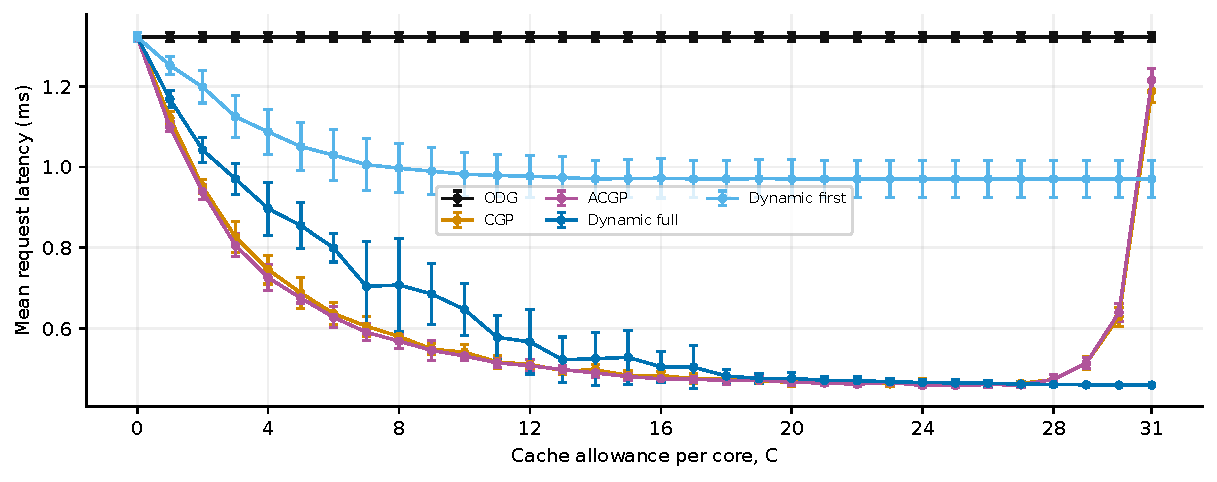
\includegraphics[width=.94\linewidth,height=.31\textheight,keepaspectratio]{figures/allocation/mesh_max_reliability_m32.pdf}\captionof{figure}{All legal C values; ODG's C=0 result is repeated as a horizontal reference, not rerun at C>0.}\end{center}
\begin{center}{\scriptsize\setlength{\tabcolsep}{3pt}
\begin{tabular}{lrrrrr}
\toprule
C & ODG & CGP & ACGP & Dynamic full & Dynamic first \\
\midrule
0 & $1.322\pm0.012$ & $1.322\pm0.012$ & $1.322\pm0.012$ & $1.322\pm0.012$ & $1.322\pm0.012$ \\
1 & $1.322\pm0.012$ & $1.122\pm0.015$ & $1.100\pm0.012$ & $1.168\pm0.021$ & $1.252\pm0.023$ \\
2 & $1.322\pm0.012$ & $0.9510\pm0.0175$ & $0.9393\pm0.0186$ & $1.043\pm0.031$ & $1.199\pm0.040$ \\
3 & $1.322\pm0.012$ & $0.8269\pm0.0382$ & $0.8064\pm0.0281$ & $0.9707\pm0.0388$ & $1.125\pm0.052$ \\
4 & $1.322\pm0.012$ & $0.7461\pm0.0358$ & $0.7262\pm0.0327$ & $0.8973\pm0.0657$ & $1.087\pm0.056$ \\
5 & $1.322\pm0.012$ & $0.6882\pm0.0383$ & $0.6755\pm0.0123$ & $0.8552\pm0.0573$ & $1.051\pm0.059$ \\
6 & $1.322\pm0.012$ & $0.6371\pm0.0270$ & $0.6280\pm0.0257$ & $0.7997\pm0.0348$ & $1.030\pm0.062$ \\
7 & $1.322\pm0.012$ & $0.6056\pm0.0250$ & $0.5909\pm0.0215$ & $0.7043\pm0.1124$ & $1.006\pm0.064$ \\
8 & $1.322\pm0.012$ & $0.5804\pm0.0126$ & $0.5687\pm0.0189$ & $0.7080\pm0.1160$ & $0.9972\pm0.0602$ \\
9 & $1.322\pm0.012$ & $0.5492\pm0.0141$ & $0.5458\pm0.0242$ & $0.6855\pm0.0765$ & $0.9898\pm0.0579$ \\
10 & $1.322\pm0.012$ & $0.5412\pm0.0187$ & $0.5321\pm0.0113$ & $0.6472\pm0.0640$ & $0.9824\pm0.0545$ \\
11 & $1.322\pm0.012$ & $0.5174\pm0.0166$ & $0.5150\pm0.0110$ & $0.5783\pm0.0542$ & $0.9793\pm0.0523$ \\
12 & $1.322\pm0.012$ & $0.5107\pm0.0135$ & $0.5077\pm0.0148$ & $0.5669\pm0.0794$ & $0.9772\pm0.0515$ \\
13 & $1.322\pm0.012$ & $0.4959\pm0.0097$ & $0.4983\pm0.0106$ & $0.5226\pm0.0565$ & $0.9742\pm0.0523$ \\
14 & $1.322\pm0.012$ & $0.4972\pm0.0126$ & $0.4900\pm0.0106$ & $0.5255\pm0.0655$ & $0.9708\pm0.0467$ \\
15 & $1.322\pm0.012$ & $0.4840\pm0.0109$ & $0.4808\pm0.0086$ & $0.5285\pm0.0664$ & $0.9715\pm0.0476$ \\
16 & $1.322\pm0.012$ & $0.4834\pm0.0095$ & $0.4755\pm0.0056$ & $0.5054\pm0.0379$ & $0.9727\pm0.0492$ \\
17 & $1.322\pm0.012$ & $0.4759\pm0.0131$ & $0.4743\pm0.0071$ & $0.5040\pm0.0532$ & $0.9707\pm0.0467$ \\
18 & $1.322\pm0.012$ & $0.4740\pm0.0034$ & $0.4714\pm0.0094$ & $0.4826\pm0.0158$ & $0.9707\pm0.0468$ \\
19 & $1.322\pm0.012$ & $0.4705\pm0.0044$ & $0.4724\pm0.0090$ & $0.4764\pm0.0124$ & $0.9713\pm0.0474$ \\
20 & $1.322\pm0.012$ & $0.4668\pm0.0110$ & $0.4667\pm0.0072$ & $0.4765\pm0.0134$ & $0.9710\pm0.0470$ \\
21 & $1.322\pm0.012$ & $0.4681\pm0.0061$ & $0.4649\pm0.0069$ & $0.4719\pm0.0089$ & $0.9706\pm0.0465$ \\
22 & $1.322\pm0.012$ & $0.4663\pm0.0043$ & $0.4621\pm0.0056$ & $0.4712\pm0.0087$ & $0.9706\pm0.0465$ \\
23 & $1.322\pm0.012$ & $0.4627\pm0.0073$ & $0.4669\pm0.0073$ & $0.4680\pm0.0071$ & $0.9706\pm0.0465$ \\
24 & $1.322\pm0.012$ & $0.4664\pm0.0095$ & $0.4588\pm0.0044$ & $0.4664\pm0.0079$ & $0.9706\pm0.0465$ \\
25 & $1.322\pm0.012$ & $0.4619\pm0.0040$ & $0.4596\pm0.0047$ & $0.4652\pm0.0077$ & $0.9706\pm0.0465$ \\
26 & $1.322\pm0.012$ & $0.4609\pm0.0067$ & $0.4610\pm0.0070$ & $0.4644\pm0.0074$ & $0.9706\pm0.0465$ \\
27 & $1.322\pm0.012$ & $0.4639\pm0.0053$ & $0.4602\pm0.0055$ & $0.4623\pm0.0056$ & $0.9706\pm0.0465$ \\
28 & $1.322\pm0.012$ & $0.4738\pm0.0128$ & $0.4742\pm0.0116$ & $0.4617\pm0.0050$ & $0.9706\pm0.0465$ \\
29 & $1.322\pm0.012$ & $0.5146\pm0.0158$ & $0.5143\pm0.0136$ & $0.4604\pm0.0022$ & $0.9706\pm0.0465$ \\
30 & $1.322\pm0.012$ & $0.6291\pm0.0239$ & $0.6400\pm0.0223$ & $0.4599\pm0.0012$ & $0.9706\pm0.0465$ \\
31 & $1.322\pm0.012$ & $1.188\pm0.027$ & $1.215\pm0.029$ & $0.4599\pm0.0011$ & $0.9706\pm0.0465$ \\
\bottomrule\end{tabular}}
\captionof{table}{Mean hop latency (ms), mean $\pm$ SD. The linked CSV includes every recorded metric for every allocation.}
{\footnotesize\href{https://github.com/sanjeevkrishnaa/Compiler-Driven-ACE/blob/codex/ace-scheduler-correctness/docs/latex/qft96_final/data/allocation_mesh_max_reliability_m32.csv}{Exact CSV values and sample counts}}
\end{center}
\section{Torus / dijkstra}
\clearpage\subsection*{M=2: every cache allowance}
\begin{center}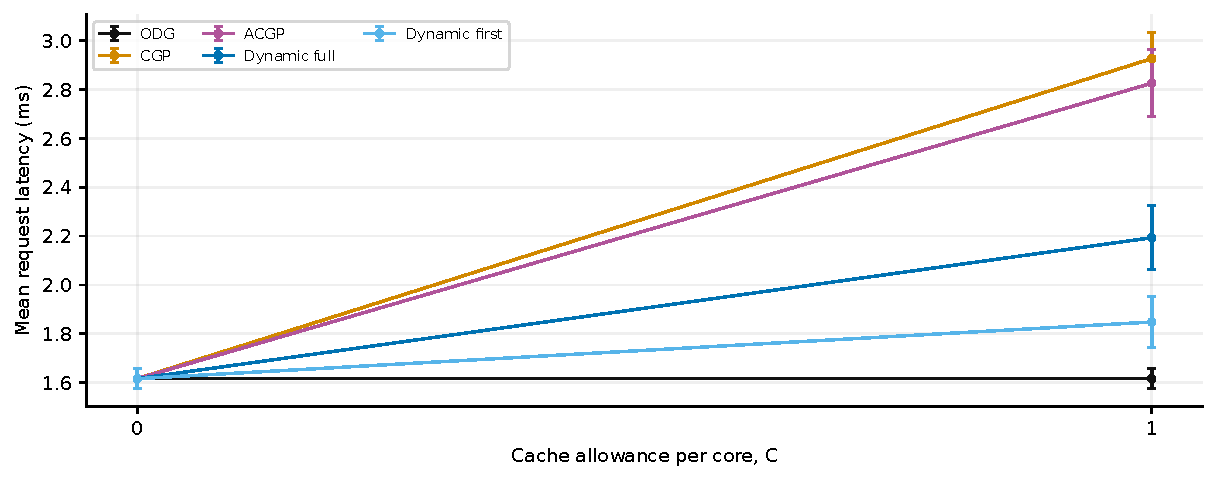
\includegraphics[width=.94\linewidth,height=.31\textheight,keepaspectratio]{figures/allocation/torus_dijkstra_m2.pdf}\captionof{figure}{All legal C values; ODG's C=0 result is repeated as a horizontal reference, not rerun at C>0.}\end{center}
\begin{center}{\scriptsize\setlength{\tabcolsep}{3pt}
\begin{tabular}{lrrrrr}
\toprule
C & ODG & CGP & ACGP & Dynamic full & Dynamic first \\
\midrule
0 & $1.616\pm0.041$ & $1.616\pm0.041$ & $1.616\pm0.041$ & $1.616\pm0.041$ & $1.616\pm0.041$ \\
1 & $1.616\pm0.041$ & $2.927\pm0.108$ & $2.826\pm0.137$ & $2.194\pm0.131$ & $1.848\pm0.105$ \\
\bottomrule\end{tabular}}
\captionof{table}{Mean hop latency (ms), mean $\pm$ SD. The linked CSV includes every recorded metric for every allocation.}
{\footnotesize\href{https://github.com/sanjeevkrishnaa/Compiler-Driven-ACE/blob/codex/ace-scheduler-correctness/docs/latex/qft96_final/data/allocation_torus_dijkstra_m2.csv}{Exact CSV values and sample counts}}
\end{center}
\clearpage\subsection*{M=3: every cache allowance}
\begin{center}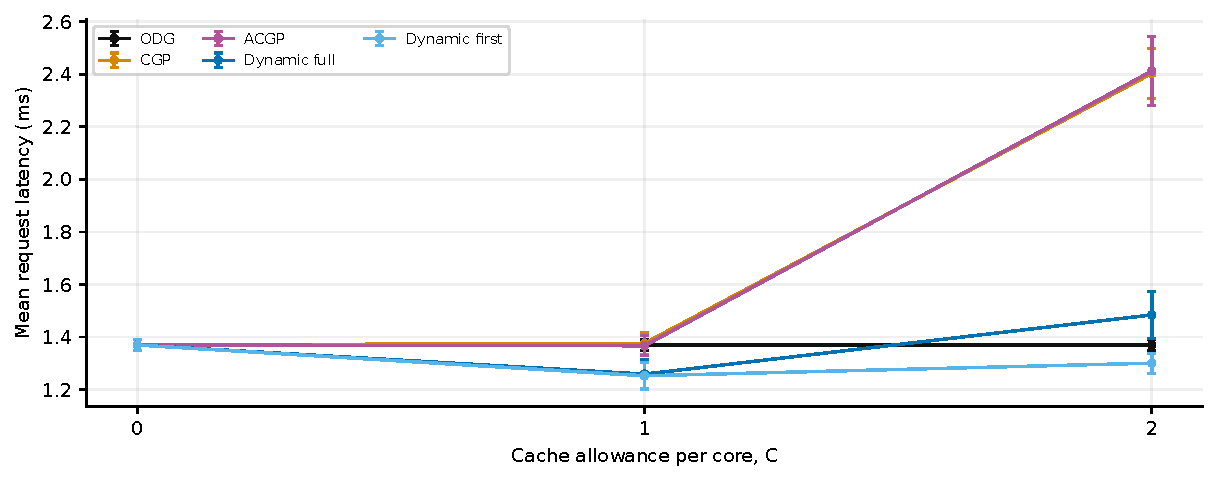
\includegraphics[width=.94\linewidth,height=.31\textheight,keepaspectratio]{figures/allocation/torus_dijkstra_m3.pdf}\captionof{figure}{All legal C values; ODG's C=0 result is repeated as a horizontal reference, not rerun at C>0.}\end{center}
\begin{center}{\scriptsize\setlength{\tabcolsep}{3pt}
\begin{tabular}{lrrrrr}
\toprule
C & ODG & CGP & ACGP & Dynamic full & Dynamic first \\
\midrule
0 & $1.370\pm0.021$ & $1.370\pm0.020$ & $1.370\pm0.020$ & $1.370\pm0.021$ & $1.370\pm0.021$ \\
1 & $1.370\pm0.021$ & $1.376\pm0.041$ & $1.367\pm0.038$ & $1.259\pm0.054$ & $1.253\pm0.050$ \\
2 & $1.370\pm0.021$ & $2.403\pm0.094$ & $2.412\pm0.130$ & $1.484\pm0.089$ & $1.301\pm0.038$ \\
\bottomrule\end{tabular}}
\captionof{table}{Mean hop latency (ms), mean $\pm$ SD. The linked CSV includes every recorded metric for every allocation.}
{\footnotesize\href{https://github.com/sanjeevkrishnaa/Compiler-Driven-ACE/blob/codex/ace-scheduler-correctness/docs/latex/qft96_final/data/allocation_torus_dijkstra_m3.csv}{Exact CSV values and sample counts}}
\end{center}
\clearpage\subsection*{M=4: every cache allowance}
\begin{center}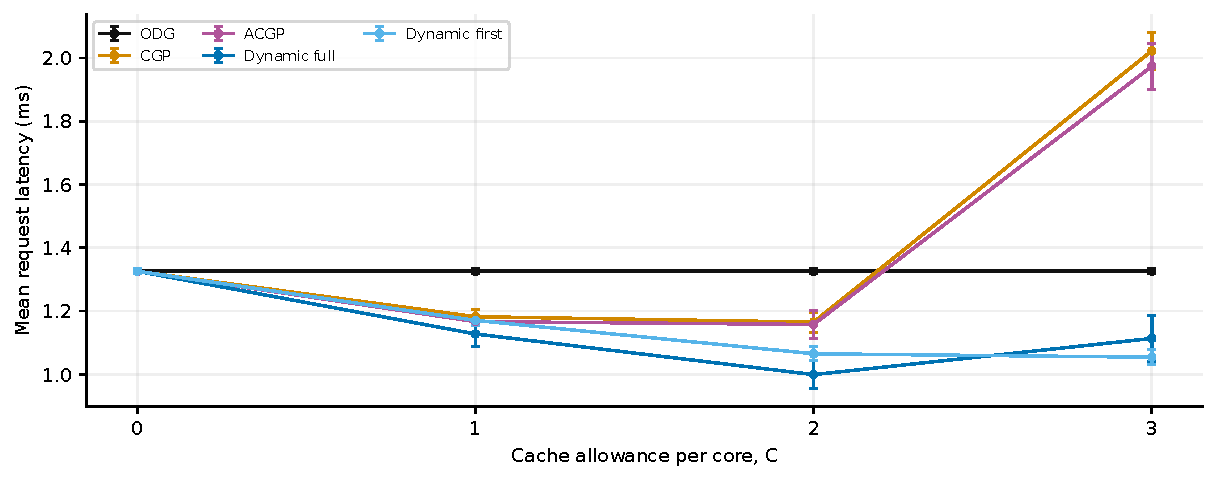
\includegraphics[width=.94\linewidth,height=.31\textheight,keepaspectratio]{figures/allocation/torus_dijkstra_m4.pdf}\captionof{figure}{All legal C values; ODG's C=0 result is repeated as a horizontal reference, not rerun at C>0.}\end{center}
\begin{center}{\scriptsize\setlength{\tabcolsep}{3pt}
\begin{tabular}{lrrrrr}
\toprule
C & ODG & CGP & ACGP & Dynamic full & Dynamic first \\
\midrule
0 & $1.326\pm0.008$ & $1.326\pm0.008$ & $1.326\pm0.008$ & $1.326\pm0.008$ & $1.326\pm0.008$ \\
1 & $1.326\pm0.008$ & $1.182\pm0.022$ & $1.167\pm0.012$ & $1.128\pm0.040$ & $1.171\pm0.016$ \\
2 & $1.326\pm0.008$ & $1.165\pm0.031$ & $1.158\pm0.044$ & $0.9992\pm0.0447$ & $1.065\pm0.023$ \\
3 & $1.326\pm0.008$ & $2.022\pm0.059$ & $1.973\pm0.072$ & $1.113\pm0.073$ & $1.054\pm0.024$ \\
\bottomrule\end{tabular}}
\captionof{table}{Mean hop latency (ms), mean $\pm$ SD. The linked CSV includes every recorded metric for every allocation.}
{\footnotesize\href{https://github.com/sanjeevkrishnaa/Compiler-Driven-ACE/blob/codex/ace-scheduler-correctness/docs/latex/qft96_final/data/allocation_torus_dijkstra_m4.csv}{Exact CSV values and sample counts}}
\end{center}
\clearpage\subsection*{M=6: every cache allowance}
\begin{center}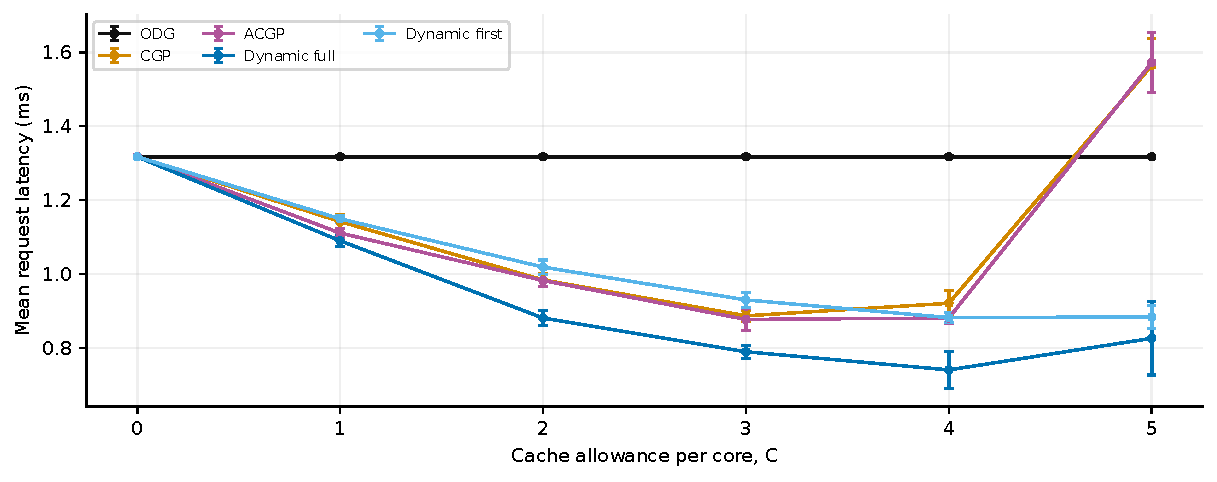
\includegraphics[width=.94\linewidth,height=.31\textheight,keepaspectratio]{figures/allocation/torus_dijkstra_m6.pdf}\captionof{figure}{All legal C values; ODG's C=0 result is repeated as a horizontal reference, not rerun at C>0.}\end{center}
\begin{center}{\scriptsize\setlength{\tabcolsep}{3pt}
\begin{tabular}{lrrrrr}
\toprule
C & ODG & CGP & ACGP & Dynamic full & Dynamic first \\
\midrule
0 & $1.317\pm0.003$ & $1.318\pm0.002$ & $1.318\pm0.002$ & $1.317\pm0.003$ & $1.317\pm0.003$ \\
1 & $1.317\pm0.003$ & $1.142\pm0.020$ & $1.111\pm0.013$ & $1.090\pm0.017$ & $1.149\pm0.009$ \\
2 & $1.317\pm0.003$ & $0.9838\pm0.0170$ & $0.9823\pm0.0171$ & $0.8807\pm0.0206$ & $1.019\pm0.019$ \\
3 & $1.317\pm0.003$ & $0.8867\pm0.0147$ & $0.8770\pm0.0308$ & $0.7895\pm0.0171$ & $0.9298\pm0.0200$ \\
4 & $1.317\pm0.003$ & $0.9207\pm0.0347$ & $0.8808\pm0.0160$ & $0.7403\pm0.0509$ & $0.8818\pm0.0143$ \\
5 & $1.317\pm0.003$ & $1.564\pm0.074$ & $1.572\pm0.082$ & $0.8259\pm0.0993$ & $0.8837\pm0.0307$ \\
\bottomrule\end{tabular}}
\captionof{table}{Mean hop latency (ms), mean $\pm$ SD. The linked CSV includes every recorded metric for every allocation.}
{\footnotesize\href{https://github.com/sanjeevkrishnaa/Compiler-Driven-ACE/blob/codex/ace-scheduler-correctness/docs/latex/qft96_final/data/allocation_torus_dijkstra_m6.csv}{Exact CSV values and sample counts}}
\end{center}
\clearpage\subsection*{M=8: every cache allowance}
\begin{center}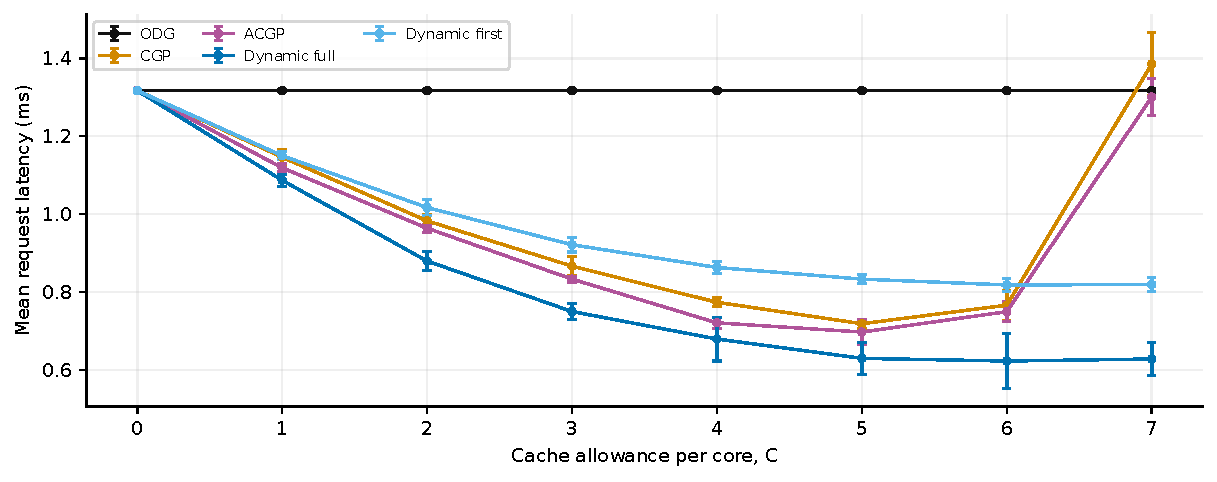
\includegraphics[width=.94\linewidth,height=.31\textheight,keepaspectratio]{figures/allocation/torus_dijkstra_m8.pdf}\captionof{figure}{All legal C values; ODG's C=0 result is repeated as a horizontal reference, not rerun at C>0.}\end{center}
\begin{center}{\scriptsize\setlength{\tabcolsep}{3pt}
\begin{tabular}{lrrrrr}
\toprule
C & ODG & CGP & ACGP & Dynamic full & Dynamic first \\
\midrule
0 & $1.317\pm0.003$ & $1.318\pm0.002$ & $1.318\pm0.002$ & $1.317\pm0.003$ & $1.317\pm0.003$ \\
1 & $1.317\pm0.003$ & $1.146\pm0.020$ & $1.119\pm0.011$ & $1.087\pm0.016$ & $1.150\pm0.010$ \\
2 & $1.317\pm0.003$ & $0.9827\pm0.0153$ & $0.9639\pm0.0101$ & $0.8795\pm0.0237$ & $1.017\pm0.020$ \\
3 & $1.317\pm0.003$ & $0.8666\pm0.0239$ & $0.8332\pm0.0077$ & $0.7501\pm0.0216$ & $0.9214\pm0.0186$ \\
4 & $1.317\pm0.003$ & $0.7739\pm0.0111$ & $0.7211\pm0.0147$ & $0.6795\pm0.0563$ & $0.8631\pm0.0160$ \\
5 & $1.317\pm0.003$ & $0.7188\pm0.0116$ & $0.6975\pm0.0311$ & $0.6299\pm0.0417$ & $0.8332\pm0.0111$ \\
6 & $1.317\pm0.003$ & $0.7665\pm0.0382$ & $0.7498\pm0.0257$ & $0.6231\pm0.0711$ & $0.8182\pm0.0157$ \\
7 & $1.317\pm0.003$ & $1.385\pm0.082$ & $1.300\pm0.048$ & $0.6283\pm0.0424$ & $0.8194\pm0.0191$ \\
\bottomrule\end{tabular}}
\captionof{table}{Mean hop latency (ms), mean $\pm$ SD. The linked CSV includes every recorded metric for every allocation.}
{\footnotesize\href{https://github.com/sanjeevkrishnaa/Compiler-Driven-ACE/blob/codex/ace-scheduler-correctness/docs/latex/qft96_final/data/allocation_torus_dijkstra_m8.csv}{Exact CSV values and sample counts}}
\end{center}
\clearpage\subsection*{M=16: every cache allowance}
\begin{center}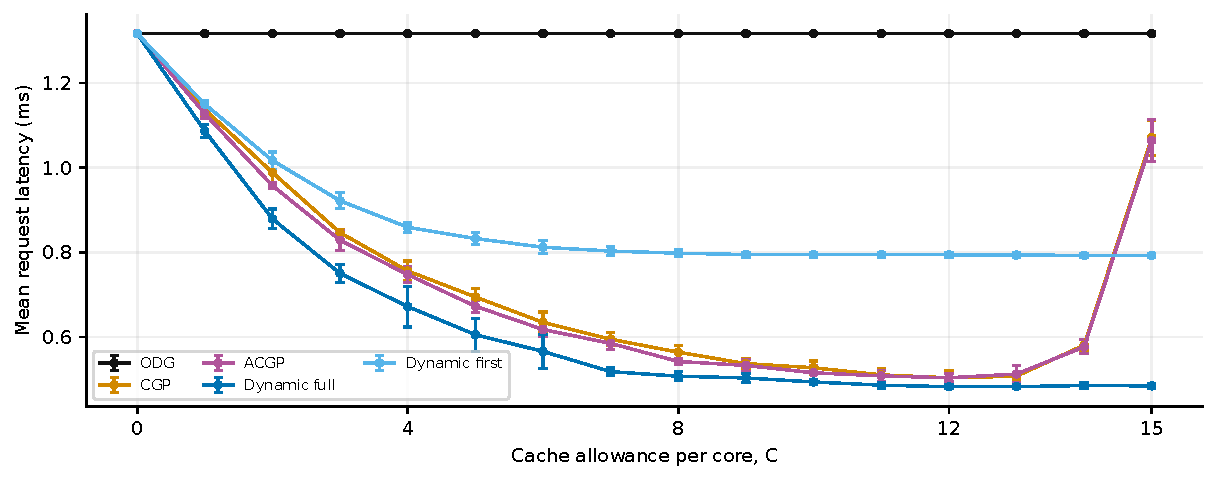
\includegraphics[width=.94\linewidth,height=.31\textheight,keepaspectratio]{figures/allocation/torus_dijkstra_m16.pdf}\captionof{figure}{All legal C values; ODG's C=0 result is repeated as a horizontal reference, not rerun at C>0.}\end{center}
\begin{center}{\scriptsize\setlength{\tabcolsep}{3pt}
\begin{tabular}{lrrrrr}
\toprule
C & ODG & CGP & ACGP & Dynamic full & Dynamic first \\
\midrule
0 & $1.317\pm0.003$ & $1.318\pm0.002$ & $1.318\pm0.002$ & $1.317\pm0.003$ & $1.317\pm0.003$ \\
1 & $1.317\pm0.003$ & $1.138\pm0.017$ & $1.127\pm0.012$ & $1.087\pm0.016$ & $1.150\pm0.010$ \\
2 & $1.317\pm0.003$ & $0.9883\pm0.0229$ & $0.9575\pm0.0066$ & $0.8789\pm0.0235$ & $1.017\pm0.020$ \\
3 & $1.317\pm0.003$ & $0.8464\pm0.0077$ & $0.8286\pm0.0233$ & $0.7501\pm0.0215$ & $0.9217\pm0.0190$ \\
4 & $1.317\pm0.003$ & $0.7560\pm0.0235$ & $0.7473\pm0.0188$ & $0.6718\pm0.0483$ & $0.8592\pm0.0123$ \\
5 & $1.317\pm0.003$ & $0.6945\pm0.0210$ & $0.6726\pm0.0137$ & $0.6054\pm0.0388$ & $0.8327\pm0.0141$ \\
6 & $1.317\pm0.003$ & $0.6343\pm0.0246$ & $0.6177\pm0.0155$ & $0.5658\pm0.0405$ & $0.8120\pm0.0151$ \\
7 & $1.317\pm0.003$ & $0.5947\pm0.0153$ & $0.5848\pm0.0147$ & $0.5181\pm0.0091$ & $0.8030\pm0.0113$ \\
8 & $1.317\pm0.003$ & $0.5639\pm0.0168$ & $0.5421\pm0.0079$ & $0.5073\pm0.0112$ & $0.7980\pm0.0087$ \\
9 & $1.317\pm0.003$ & $0.5370\pm0.0121$ & $0.5327\pm0.0151$ & $0.5031\pm0.0109$ & $0.7947\pm0.0059$ \\
10 & $1.317\pm0.003$ & $0.5272\pm0.0161$ & $0.5153\pm0.0160$ & $0.4936\pm0.0050$ & $0.7944\pm0.0058$ \\
11 & $1.317\pm0.003$ & $0.5103\pm0.0162$ & $0.5080\pm0.0126$ & $0.4861\pm0.0067$ & $0.7945\pm0.0061$ \\
12 & $1.317\pm0.003$ & $0.5034\pm0.0180$ & $0.5035\pm0.0096$ & $0.4824\pm0.0048$ & $0.7943\pm0.0061$ \\
13 & $1.317\pm0.003$ & $0.5074\pm0.0076$ & $0.5125\pm0.0207$ & $0.4826\pm0.0049$ & $0.7934\pm0.0050$ \\
14 & $1.317\pm0.003$ & $0.5806\pm0.0128$ & $0.5767\pm0.0165$ & $0.4853\pm0.0071$ & $0.7929\pm0.0050$ \\
15 & $1.317\pm0.003$ & $1.071\pm0.041$ & $1.064\pm0.050$ & $0.4844\pm0.0056$ & $0.7930\pm0.0051$ \\
\bottomrule\end{tabular}}
\captionof{table}{Mean hop latency (ms), mean $\pm$ SD. The linked CSV includes every recorded metric for every allocation.}
{\footnotesize\href{https://github.com/sanjeevkrishnaa/Compiler-Driven-ACE/blob/codex/ace-scheduler-correctness/docs/latex/qft96_final/data/allocation_torus_dijkstra_m16.csv}{Exact CSV values and sample counts}}
\end{center}
\clearpage\subsection*{M=32: every cache allowance}
\begin{center}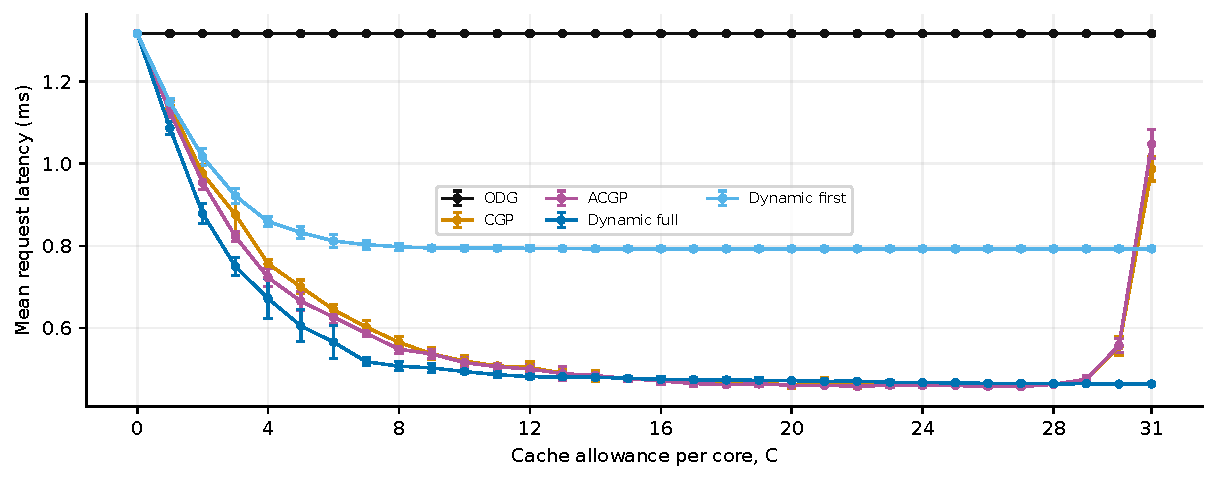
\includegraphics[width=.94\linewidth,height=.31\textheight,keepaspectratio]{figures/allocation/torus_dijkstra_m32.pdf}\captionof{figure}{All legal C values; ODG's C=0 result is repeated as a horizontal reference, not rerun at C>0.}\end{center}
\begin{center}{\scriptsize\setlength{\tabcolsep}{3pt}
\begin{tabular}{lrrrrr}
\toprule
C & ODG & CGP & ACGP & Dynamic full & Dynamic first \\
\midrule
0 & $1.317\pm0.003$ & $1.318\pm0.002$ & $1.318\pm0.002$ & $1.317\pm0.003$ & $1.317\pm0.003$ \\
1 & $1.317\pm0.003$ & $1.143\pm0.010$ & $1.126\pm0.012$ & $1.087\pm0.016$ & $1.150\pm0.010$ \\
2 & $1.317\pm0.003$ & $0.9755\pm0.0225$ & $0.9548\pm0.0182$ & $0.8789\pm0.0235$ & $1.017\pm0.020$ \\
3 & $1.317\pm0.003$ & $0.8765\pm0.0429$ & $0.8230\pm0.0119$ & $0.7501\pm0.0215$ & $0.9217\pm0.0190$ \\
4 & $1.317\pm0.003$ & $0.7565\pm0.0113$ & $0.7228\pm0.0222$ & $0.6718\pm0.0483$ & $0.8592\pm0.0123$ \\
5 & $1.317\pm0.003$ & $0.7002\pm0.0168$ & $0.6655\pm0.0234$ & $0.6054\pm0.0388$ & $0.8327\pm0.0141$ \\
6 & $1.317\pm0.003$ & $0.6448\pm0.0121$ & $0.6266\pm0.0161$ & $0.5658\pm0.0405$ & $0.8120\pm0.0151$ \\
7 & $1.317\pm0.003$ & $0.6022\pm0.0159$ & $0.5873\pm0.0083$ & $0.5181\pm0.0091$ & $0.8030\pm0.0113$ \\
8 & $1.317\pm0.003$ & $0.5653\pm0.0133$ & $0.5486\pm0.0114$ & $0.5073\pm0.0112$ & $0.7980\pm0.0087$ \\
9 & $1.317\pm0.003$ & $0.5372\pm0.0143$ & $0.5369\pm0.0116$ & $0.5031\pm0.0109$ & $0.7947\pm0.0059$ \\
10 & $1.317\pm0.003$ & $0.5198\pm0.0134$ & $0.5160\pm0.0125$ & $0.4942\pm0.0052$ & $0.7944\pm0.0058$ \\
11 & $1.317\pm0.003$ & $0.5078\pm0.0041$ & $0.5059\pm0.0069$ & $0.4867\pm0.0076$ & $0.7945\pm0.0061$ \\
12 & $1.317\pm0.003$ & $0.5043\pm0.0132$ & $0.5003\pm0.0098$ & $0.4816\pm0.0044$ & $0.7943\pm0.0061$ \\
13 & $1.317\pm0.003$ & $0.4900\pm0.0094$ & $0.4892\pm0.0174$ & $0.4814\pm0.0045$ & $0.7934\pm0.0050$ \\
14 & $1.317\pm0.003$ & $0.4828\pm0.0129$ & $0.4845\pm0.0037$ & $0.4805\pm0.0058$ & $0.7929\pm0.0050$ \\
15 & $1.317\pm0.003$ & $0.4773\pm0.0052$ & $0.4770\pm0.0062$ & $0.4777\pm0.0040$ & $0.7928\pm0.0050$ \\
16 & $1.317\pm0.003$ & $0.4730\pm0.0079$ & $0.4714\pm0.0078$ & $0.4752\pm0.0058$ & $0.7928\pm0.0050$ \\
17 & $1.317\pm0.003$ & $0.4679\pm0.0101$ & $0.4649\pm0.0076$ & $0.4742\pm0.0055$ & $0.7928\pm0.0050$ \\
18 & $1.317\pm0.003$ & $0.4680\pm0.0059$ & $0.4624\pm0.0039$ & $0.4736\pm0.0067$ & $0.7928\pm0.0050$ \\
19 & $1.317\pm0.003$ & $0.4680\pm0.0108$ & $0.4641\pm0.0072$ & $0.4729\pm0.0060$ & $0.7928\pm0.0050$ \\
20 & $1.317\pm0.003$ & $0.4601\pm0.0075$ & $0.4609\pm0.0025$ & $0.4721\pm0.0023$ & $0.7928\pm0.0050$ \\
21 & $1.317\pm0.003$ & $0.4695\pm0.0110$ & $0.4607\pm0.0025$ & $0.4706\pm0.0031$ & $0.7928\pm0.0050$ \\
22 & $1.317\pm0.003$ & $0.4620\pm0.0097$ & $0.4584\pm0.0031$ & $0.4707\pm0.0025$ & $0.7928\pm0.0050$ \\
23 & $1.317\pm0.003$ & $0.4619\pm0.0031$ & $0.4607\pm0.0052$ & $0.4682\pm0.0037$ & $0.7928\pm0.0050$ \\
24 & $1.317\pm0.003$ & $0.4606\pm0.0034$ & $0.4604\pm0.0049$ & $0.4671\pm0.0025$ & $0.7928\pm0.0050$ \\
25 & $1.317\pm0.003$ & $0.4607\pm0.0035$ & $0.4601\pm0.0029$ & $0.4668\pm0.0029$ & $0.7928\pm0.0050$ \\
26 & $1.317\pm0.003$ & $0.4619\pm0.0037$ & $0.4583\pm0.0029$ & $0.4654\pm0.0021$ & $0.7928\pm0.0050$ \\
27 & $1.317\pm0.003$ & $0.4625\pm0.0042$ & $0.4576\pm0.0021$ & $0.4653\pm0.0024$ & $0.7928\pm0.0050$ \\
28 & $1.317\pm0.003$ & $0.4631\pm0.0015$ & $0.4631\pm0.0027$ & $0.4645\pm0.0020$ & $0.7928\pm0.0050$ \\
29 & $1.317\pm0.003$ & $0.4757\pm0.0051$ & $0.4757\pm0.0082$ & $0.4645\pm0.0025$ & $0.7928\pm0.0050$ \\
30 & $1.317\pm0.003$ & $0.5558\pm0.0225$ & $0.5579\pm0.0170$ & $0.4638\pm0.0019$ & $0.7928\pm0.0050$ \\
31 & $1.317\pm0.003$ & $0.9872\pm0.0292$ & $1.048\pm0.035$ & $0.4640\pm0.0023$ & $0.7928\pm0.0050$ \\
\bottomrule\end{tabular}}
\captionof{table}{Mean hop latency (ms), mean $\pm$ SD. The linked CSV includes every recorded metric for every allocation.}
{\footnotesize\href{https://github.com/sanjeevkrishnaa/Compiler-Driven-ACE/blob/codex/ace-scheduler-correctness/docs/latex/qft96_final/data/allocation_torus_dijkstra_m32.csv}{Exact CSV values and sample counts}}
\end{center}